\documentclass[draft]{agujournal2019}
\usepackage{url} %this package should fix any errors with URLs in refs.
\usepackage{lineno}
%\usepackage[inline]{trackchanges} %for better track changes. finalnew option will compile document with changes incorporated.
\usepackage{soul}
\linenumbers

\draftfalse

\journalname{JGR: Atmospheres}

\begin{document}

\title{Ship-based lidar evaluation of Southern Ocean clouds in the storm-resolving general circulation model ICON, and the ERA5 and MERRA-2 reanalyses}

\authors{Peter Kuma\affil{1,2}\thanks{}, Frida A.-M. Bender\affil{1,2}, Adrian J. McDonald\affil{3}, Simon P. Alexander\affil{4,5}, Greg M. McFarquhar\affil{6,7}, John J. Cassano\affil{8,9,10}, Graeme E. Plank\affil{3}, Sean Hartery\affil{11}, Simon Parsons\affil{12}, Sally Garrett\affil{13}, and Alex J. Schuddeboom\affil{3}}

\affiliation{1}{Department of Meteorology (MISU), Stockholm University, Stockholm, Sweden}
\affiliation{2}{Bolin Centre for Climate Research, Stockholm University, Stockholm, Sweden}
\affiliation{3}{School of Physical and Chemical Sciences, University of Canterbury, Christchurch, Aotearoa/New Zealand}
\affiliation{4}{Australian Antarctic Division, Kingston, Tasmania, Australia}
\affiliation{5}{Australian Antarctic Program Partnership, Institute for Marine and Antarctic Studies, University of Tasmania, Hobart, Tasmania, Australia}
\affiliation{6}{Cooperative Institute of Severe and High Impact Weather Research and Operations, University of Oklahoma, Norman, OK, USA}
\affiliation{7}{School of Meteorology, University of Oklahoma, Norman, OK, USA}
\affiliation{8}{Cooperative Institute for Research in Environmental Sciences, University of Colorado, Boulder, CO, USA}
\affiliation{9}{National Snow and Ice Data Center, University of Colorado, Boulder, CO, USA}
\affiliation{10}{Department of Atmospheric and Oceanic Sciences, University of Colorado, Boulder, CO, USA}
\affiliation{11}{Department of Physics \& Atmospheric Science, Dalhousie University, Halifax, Canada}
\affiliation{12}{New South Wales Department of Planning and Environment, Sydney, New South Wales, Australia}
\affiliation{13}{New Zealand Defence Force, Wellington, Aotearoa/New Zealand}

\correspondingauthor{Peter Kuma}{peter@peterkuma.net}

\begin{keypoints}
\item Ground-based lidar evaluation of a km-scale global climate model and reanalyses reveals substantial cloud biases over the Southern Ocean.
\item Fog or low cloud is underestimated in the reanalyses. In all models, a cloud peak at 500~m tends to be overestimated and too high.
\item A ``too few, too bright'' problem of underestimated cloud fraction, compensated by overestimated cloud albedo, is present in the reanalyses.
\end{keypoints}

\begin{abstract}
Global storm-resolving models (GSRMs) are the upcoming global climate models. One of them is a 5-km Icosahedral Nonhydrostatic Weather and Climate Model (ICON). The high resolution means that parameterizations of convection and clouds, including subgrid-scale clouds, are omitted, relying on explicit simulation but still utilizing microphysics and turbulence parameterizations. Standard-resolution (10--100~km) models, which use convection and cloud parameterizations, have substantial cloud biases over the Southern Ocean (SO), affecting radiation and sea surface temperature. The SO is dominated by low clouds, which cannot be observed accurately from space due to overlapping clouds, attenuation, and ground clutter. We evaluated SO clouds in ICON and the ERA5 and MERRA-2 reanalyses using about 2400 days of lidar observations and 2300 radiosonde profiles from 31 voyages and a station during 2010--2021, compared with the models using a ground-based lidar simulator. We found that ICON and the reanalyses underestimate the total cloud fraction by about 10 and 20\%, respectively. ICON and ERA5 overestimate the cloud occurrence peak at about 500 m, potentially explained by their lifting condensation levels being too high. The reanalyses strongly underestimate fog or near-surface clouds, and MERRA-2 underestimates cloud occurrence at almost all heights. Outgoing shortwave radiation is overestimated in the reanalyses, implying a ``too few, too bright'' cloud problem. Thermodynamic conditions are relatively well represented, but ICON is less stable than observations and MERRA-2 is too humid. SO cloud biases are a substantial issue in the GSRM, but it matches the observations better than the lower-resolution reanalyses.
\end{abstract}

\section*{Plain Language Summary}

Global storm-resolving models are climate models with km-scale horizontal resolution, which are currently in development. Reanalyses are the best estimates of past meteorological conditions based on an underlying global model and observations. We evaluated clouds and thermodynamic profiles over the Southern Ocean in one such model, as well as two reanalyses, based on 2400 days of ship and station observations. Thanks to the high resolution, the model relies entirely on explicit simulation of clouds, instead of subgrid-scale parameterizations. For the evaluation, we used ceilometer and radiosonde observations and a lidar simulator, which enables a fair comparison with the model and reanalyses. We subsetted our results by cyclonic activity and stability. We found that the model and reanalyses underestimate a lidar-derived cloud fraction, and the reanalyses do so more strongly. Fog or near-surface clouds are especially underestimated in the reanalyses. However, the model and one of the reanalyses also tend to overestimate the peak of cloud occurrence at 500 m above the ground, and it tends to be higher. This is linked to thermodynamic profiles, which show a higher lifting condensation level. Southern Ocean biases are still an important problem in the model, but an improvement over the reanalyses is notable.

\section{Introduction}
\label{sec:introduction}

Increasing climate model resolution is one way of improving model accuracy of representation of the climate system \cite{mauritsen2022}. It has been practiced since the advent of climate modeling as more computational power, memory, and storage capacity become available. It is, however, often not as easy as changing the grid size because of the complex interplay between model dynamics and physics, which necessitates adjusting and tuning all components together. Increasing resolution is, of course, limited by the available computational power and a trade-off with increasing parameterization complexity, which is another way of improving model accuracy. Current computational availability and acceleration from general-purpose computing on graphics processing units (GPUs) is progressing to enable km-scale (also called k-scale) Earth system models (ESMs) and coupled atmosphere--ocean general circulation models (AOGCMs) in research conditions today and operationally in the forthcoming years. Therefore, it represents a natural advance in climate modeling. Global storm-resolving models (GSRMs) are emerging as a new front in the development of high-resolution global climate models, with horizontal grid resolutions of about 2--8~km \cite{satoh2019,stevens2019}. This is enough to resolve mesoscale convective storms, but smaller-scale convective plumes and cloud structure remain unresolved. At an approximately 5-km scale, non-hydrostatic processes also become important \cite{weisman1997}, and for this reason such models are generally non-hydrostatic. The terms global cloud-resolving models or global convection-permitting/-resolving models are also sometimes used interchangeably with GSRMs but imply that clouds or convection are resolved explicitly, which is not entirely true for GSRMs, as this would require an even higher horizontal resolution \cite{satoh2019}. Representative of these efforts is the DYnamics of the Atmospheric general circulation Modeled On Non-hydrostatic Domains (DYAMOND) project \cite{stevens2019,dyamond}, which is an intercomparison of nine global GSRMs over two 40-day time periods in summer (1~August--10~September 2016) and winter (20~January--1~March 2020). A new one-year GSRM intercomparison is currently proposed by \citeA{takasuka2024}, with the hope of also evaluating the seasonal cycle and large-scale circulation. An alternative to using a computationally costly GSRM is to train an artificial neural network on GSRM output and use it for subgrid-scale clouds, as done with the GSRM ICON by \citeA{grundner2022} and \citeA{grundner2023}.

nextGEMS is a project \cite{nextgems} focused on the research and development of GSRMs at multiple modeling centers and universities in Europe. The project also develops GSRM versions of the Icosahedral Nonhydrostatic Weather and Climate Model (ICON; \citeA{hohenegger2023}), the Integrated Forecasting System [IFS; \citeA{ifs2023}], and their ocean components at eddy-resolving resolutions: ICON-O \cite{korn2022} coupled with ICON and Finite-Element/volumE Sea ice-Ocean Model [FESOM; \citeA{wang2014a}] and Nucleus for European modeling of the Ocean [NEMO; \citeA{madec2023}] coupled with IFS. The project has so far produced ICON and IFS simulations with three development versions called Cycle 1--3 and a pre-final version, with a final production version planned by the end of the project. nextGEMS is not the only project developing GSRMs; other GSRMs (or GSRM versions of climate models) currently in development include: Convection-Permitting Simulations With the E3SM Global Atmosphere Model [SCREAM; \citeA{caldwell2021}], Atmospheric Model [NICAM; \citeA{satoh2008}], Unified Model (UM), eXperimental System for High-resolution modeling for Earth-to-Local Domain [X-SHiELD; \citeA{shield}], Action de Recherche Petite Echelle Grande Echelle-NonHydrostatic version [ARPEGE-NH; \citeA{bubnova1995,voldoire2017}], Finite-Volume Dynamical Core on the Cubed Sphere [FV3, \citeA{lin2004}], the National Aeronautics and Space Administration (NASA) Goddard Earth Observing System global atmospheric model version 5 [GEOS5; \citeA{putman2011}], Model for Prediction Across Scales [MPAS; \citeA{skamarock2012}], and System for Atmospheric Modeling [SAM; \citeA{khairoutdinov2003}].

Multiple cloud properties have an effect on shortwave (SW) and longwave (LW) radiation. To first order, the total cloud fraction, cloud phase, and the liquid and ice water path are the most important cloud properties influencing SW and LW radiation. These properties are in turn influenced by the atmospheric thermodynamics, convection and circulation, and both the indirect and direct effects of aerosols. Second-order effects on SW and LW radiation are associated with the cloud droplet size distribution, ice crystal habit, cloud lifetime, and direct radiative interaction with aerosols. In the 6$^\mathrm{th}$ phase of the Coupled Model Intercomparison Project [CMIP6; \citeA{eyring2016}], the cloud feedback has increased relative to CMIP5 \cite{zelinka2020}, which is one of the main reasons for the higher climate sensitivity of CMIP6 models.

The Southern Ocean (SO) is known to be a problematic region for climate model biases \cite{schuddeboom2021,hyder2018,cesana2022,zhao2022} due to a lack of surface and in situ observations and being a lower priority region for numerical weather prediction (NWP) and climate model development because of its distance from populated areas. Nevertheless, radiation biases and changes over an area of its size have a substantial influence on the global climate \cite{rintoul2011}, such as affecting the Earth radiation balance, ocean heat, and carbon uptake \cite{williams2023}, and the SO is an important part of the global ocean conveyor belt \cite{wang2014b}. In general, marine clouds have a disproportionate effect on top of atmosphere (TOA) SW radiation due to the relatively low albedo of the sea surface. The relative longitudinal symmetry of the SO means that model cloud biases tend to be similar across longitudes.

Here, we conventionally refer to the SO as ocean regions south of 40°S, low-latitude SO as 40--55°S and high-latitude SO as south of 55°S. The reason for this dividing latitude is to split the SO into about two equal zones, as well as the results by \citeA{schuddeboom2021} (Fig.~2b), showing a contrast in CMIP model radiation biases, \citeA{schuddeboom2019} (Fig.~2) and \citeA{kuma2020} (Fig.~3) showing contrasting radiation biases in the Hadley Centre Global Environmental Model, and \citeA{cesana2022} showing contrasting cloud biases due to the 0°C isotherm reaching the surface at 55°S. The findings of \citeA{niu2024}, however, support a different dividing line of 62°S based on cloud condensation nuclei concentration.

SO radiation biases have been relatively large and systematic compared to the rest of the globe since at least CMIP3 \cite{trenberth2010}, and the SO SW cloud radiative effect (CRE) bias is still positive in eight analyzed CMIP6 models analyzed by \citeA{schuddeboom2021} over the high-latitude SO, whereas over the low-latitude SO it tends to be more neutral or negative in some models. Too much absorbed SW radiation over the SO was also identified in the GSRM SCREAM \cite{caldwell2021}. Compensating biases are possible, such as the ``too few too bright'' cloud bias, characterized by too small cloud fraction and too large cloud albedo \cite{wall2017,kuma2020}, previously described by \citeA{webb2001}, \citeA{weare2004}, \citeA{zhang2005}, \citeA{karlsson2008}, \citeA{nam2012}, \citeA{klein2013}, and \citeA{bender2017} in other regions and models, which means that a model can maintain a reasonable SW radiation balance by reflecting too much SW radiation from clouds, but these cover too small an area. A study by \citeA{konsta2022} showed that this type of bias is still present in six analyzed CMIP6 models in tropical marine clouds, using the GCM-Oriented Cloud-Aerosol Lidar and Infrared Pathfinder Satellite Observation (CALIPSO) Cloud Product [CALIPSO--GOCCP; \citeA{chepfer2010}] and Polarization \& Anisotropy of Reflectances for Atmospheric Sciences coupled with Observations from a Lidar [PARASOL; \citeA{lier2008}] as a reference. They suggest improper simulation of subgrid-scale cloud heterogeneity as a cause. Compensating cloud biases in the Australian Community Climate and Earth System Simulator (ACCESS) – Atmosphere-only model version 2 (AM2) over the SO were analyzed by \citeA{fiddes2022} and \citeA{fiddes2024}. \citeA{possner2022} showed that over the SO, the DYAMOND GSRM ICON underestimates low-level cloud fraction on the order of 30\% and overestimates net downward TOA SW radiation by approximately 10 Wm$^\mathrm{-2}$ in the highest model resolution run (2.5~km). \citeA{zhao2022} reported a similar SW radiation bias in five analyzed CMIP6 models over high-latitude SO and the total cloud fraction underestimation on the order of 10\% over the entire 40--60°S SO. Recently, \citeA{ramadoss2024} analyzed 48~hours of km-scale ICON limited-area model NWP simulations over a SO region adjacent to Tasmania against the Clouds, Aerosols, Precipitation, Radiation, and atmospherIc Composition Over the southeRn oceaN (CAPRICORN) voyage cloud and precipitation observations \cite{mcfarquhar2021}. They found the ICON cloud optical thickness was underestimated relative to Himawari‐8 satellite observations but also identified large differences in cloud top phase.

In general, sea surface temperature (SST) biases in the SO can originate either in the atmosphere \cite{hyder2018}, caused by too much shortwave heating of the surface, too little longwave cooling of the surface, or in the ocean circulation. Interactions of both are also possible, for example, SST affecting clouds and clouds affecting the surface radiation. Using the European Centre for Medium-Range Weather Forecasts (ECMWF) Reanalysis 5 (ERA5) as a reference, \citeA{zhang2023} have shown that SST biases have improved in CMIP6 compared to CMIP5, with SST overall increasing in the later CMIP phase. However, over the SO this resulted in an even higher positive bias, especially in the Atlantic Ocean (AO) sector of the SO, increasing by up to 1°C. \citeA{luo2023} identified that the SO SST bias in an ensemble of 18 CMIP6 models originates not from the surface heat and radiation fluxes (using reanalyses as a reference), but from a warm bias in the Northern Atlantic Deep Water.

The main aim of this study is to evaluate the GSRM version of ICON. ICON is developed and maintained jointly by Deutscher Wetterdienst, Max-Planck-Institute for Meteorology, Deutsches Klimarechenzentrum (DKRZ), Karlsruhe Institute of Technology, and the Center for Climate Systems Modeling. Previous studies have identified substantial large-scale biases in climate model clouds over the SO, affecting sea surface temperature and the Earth’s albedo. Our aim is to quantify how well the GSRM ICON is simulating clouds in this region, particularly in light of the fact that subgrid-scale clouds and convection are not parameterized in this model. This region is mostly dominated by boundary layer clouds generated by shallow convection, and these are problematic to observe by spaceborne lidars and radars, which are affected by attenuation by overlapping and thick clouds \cite{mace2009,medeiros2010} and ground clutter \cite{marchand2008}, respectively. Specifically, the radar on CloudSat and lidar on CALIPSO (neither of which are now operational) are affected by the abovementioned issues, resulting in a strong underestimation of cloud occurrence below 2 km relative to ground-based lidar observations \cite{mcerlich2021}. We hypothesize that this, in turn, can lead to systematic biases in low clouds in climate models, which are frequently evaluated against CloudSat--CALIPSO products. Reanalyses can also suffer from cloud biases, as these are usually parameterized in their atmospheric component and also in regions where input observations are sparse. This makes them a problematic reference for clouds over the SO, and any biases relative to a reanalysis should be interpreted with caution. Instead, we chose to use a large set of ship-based observations conducted with ceilometers and lidars on board the RV \emph{Polarstern} and other voyages and stations as a reference for the model evaluation.

Altogether, we analyzed about 2400 days of data from 31 voyages and one sub-Antarctic station covering diverse longitudes and latitudes of the SO. To achieve a like-for-like comparison with the model, we used a ground-based lidar simulator called the Automatic Lidar and Ceilometer Framework [ALCF; \citeA{kuma2021}]. We contrasted the results with ERA5 \cite{era5} and the Modern-Era Retrospective analysis for Research and Applications, Version~2 [MERRA-2; \citeA{gelaro2017}].

\begin{figure}[b!]
\centering
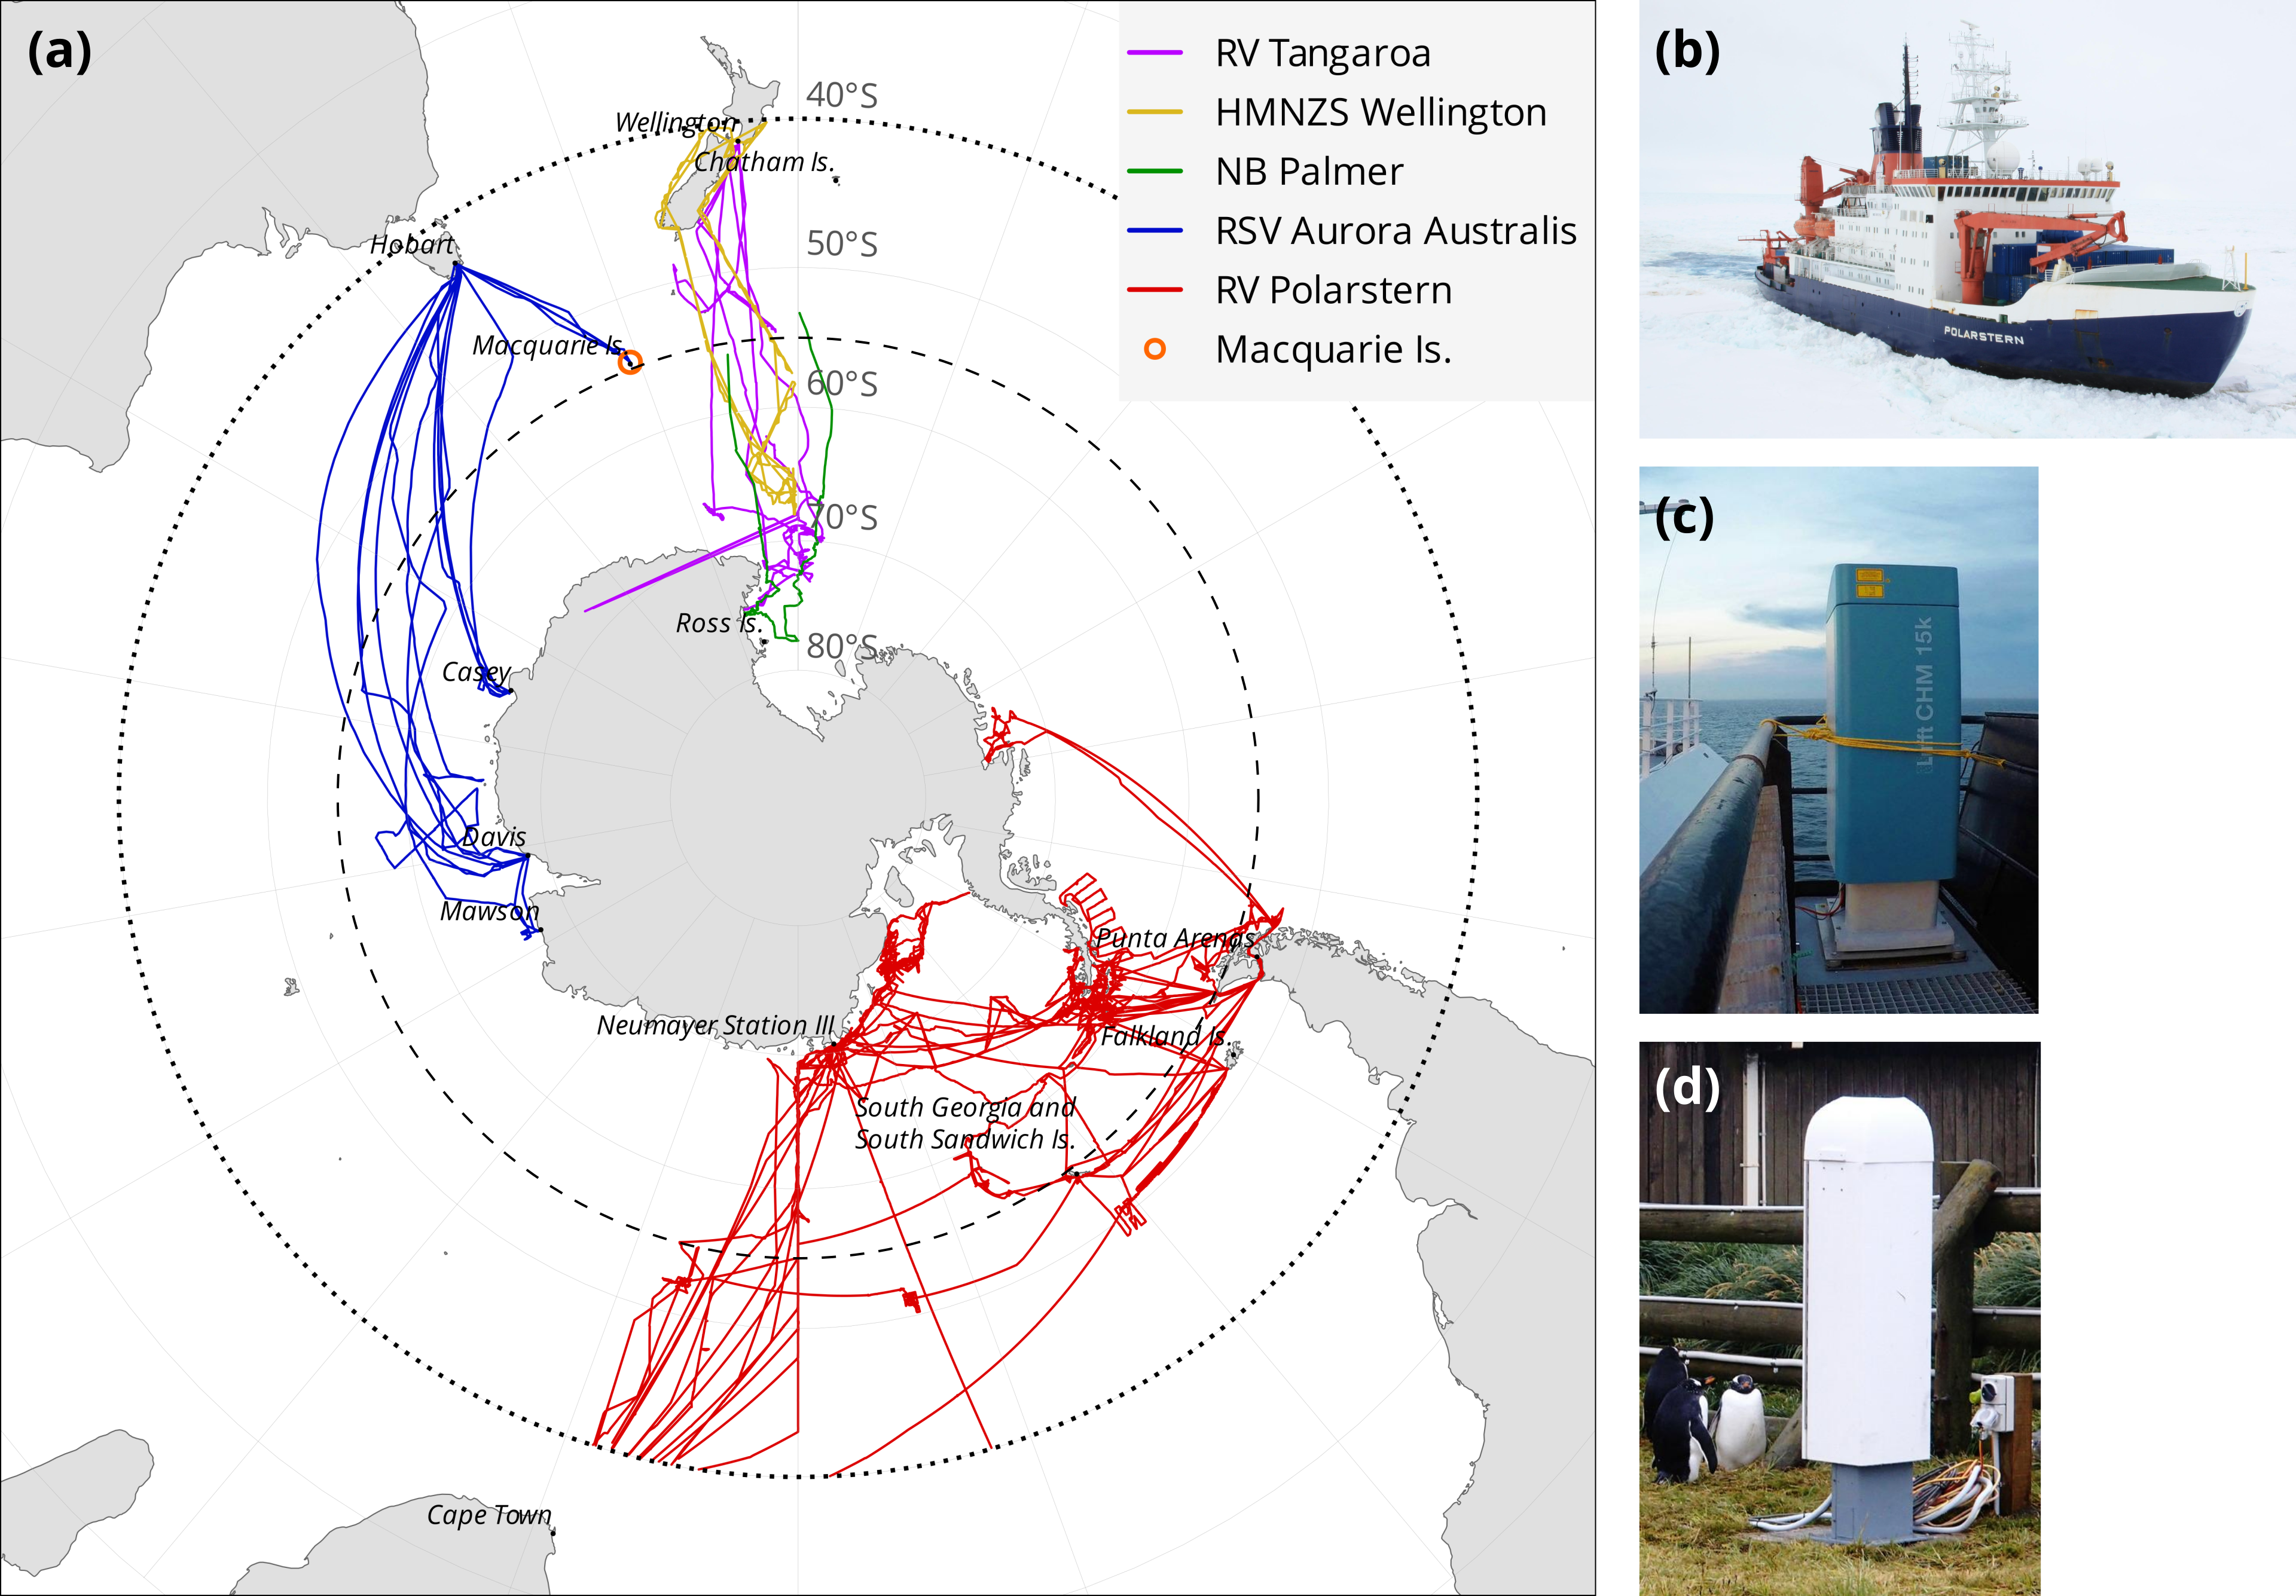
\includegraphics[width=\textwidth]{img/map_fig.pdf}
\caption{
\textbf{(a)} A map showing the tracks of 31 voyages of RV \emph{Polarstern}, RSV \emph{Aurora Australis}, RV \emph{Tangaroa}, RV \emph{Nathaniel B. Palmer}, and HMNZS \emph{Wellington} and one sub-Antarctic station (Macquarie Island) analyzed here. The tracks cover Antarctic sectors south of South America, the Atlantic Ocean, Africa, Australia, and New Zealand in the years 2010--2021 (inclusive). The dotted and dashed lines at 40°S and 55°S delineate the Southern Ocean area of our analysis and its partitioning into two subsets, respectively. A photo of \textbf{(b)} RV \emph{Polarstern} (© Folke Mehrtens, Alfred-Wegener-Institut), \textbf{(c)} Lufft CHM~15k installed on RV \emph{Tangaroa} (© Peter Kuma, University of Canterbury), \textbf{(d)} Vaisala CL51 (© Jeff Aquilina, Bureau of Meteorology), \textbf{(e)} Vaisala CT25K at Macquarie Island (© Simon P.\ Alexander, Australian Antarctic Division).
}
\label{fig:map}
\end{figure}

\section{Methods}
\label{sec:methods}

\subsection{Voyage and Station Data}

Together, we analyzed data from 31 voyages of RV \emph{Polarstern}, the resupply vessel (RSV) \emph{Aurora Australis}, RV \emph{Tangaroa}, RV \emph{Nathaniel B. Palmer}, Her (now His) Majesty's New Zealand Ship (HMNZS) \emph{Wellington} and one sub-Antarctic station (Macquarie Island) in the SO south of 40°S between 2010 and 2021. Fig.~\ref{fig:map} shows a map of the campaigns, Table \ref{tab:voyages} lists the campaigns, and Table \ref{tab:voyage-references} lists references where available. Altogether, the analyzed dataset comprised 2421 days of data south of 40°S, but the availability of ceilometer data was slightly shorter due to gaps in measurements.

The campaigns contained ceilometer observations captured by the Vaisala CL51 and CT25K, and the Lufft CHM~15k, described in detail below (Sections~\ref{sec:cl51} and \ref{sec:chm15k}). A ceilometer is a low-power, near-infrared, vertically pointing lidar principally designed to measure cloud base, but they also measure the full vertical structure of clouds as long as the laser signal is not attenuated by thick clouds, which can be used to infer additional information such as a cloud mask and cloud occurrence by height. We note that during the MICRE campaign, the ceilometers Vaisala CT25K and CL51 were installed at the Macquarie Island station concurrently, but in our analysis we only used the CT25K data obtained from the Atmospheric Radiation Measurement (ARM) data archive.

Apart from lidar observations, radiosondes were launched on weather balloons at regular synoptic times on the RV \emph{Polarstern}, MARCUS, NBP17024, TAN1702, and TAN1802 campaigns, measuring pressure, temperature, relative humidity, and the global navigation satellite system coordinates. Derived thermodynamic (virtual potential temperature, lifting condensation level, etc.) and dynamic physical quantities (wind speed and direction) for the measured vertical profiles were calculated with rstool \cite{rstool}. Surface meteorological quantities were measured continuously by an onboard automatic weather station or individual instruments.

\begin{table}[p!]
\caption{
An overview of the analyzed campaigns (voyages and stations). Start, end, and the number of days (UTC; inclusive) refer to the time period when the vessel was south of 40°S. Abbreviations: ceilometer (ceil.), Australia (AU), New Zealand (NZ), South America (SA), Atlantic Ocean (AO), and Africa (AF). The number of days is rounded to the nearest integer. CL51/31 indicates CL51 configured to emulate CL31. Missing days in the ceilometer data were HMNZSW16 (7 days): 24--27 November, 10~December, 16--17~December 2016; MARCUS (3 days): 8, 10~November, 10~December 2017; MICRE (9~days): 7--8, 29~June, 5, 16~July, 15~August, 17~October 2016, 11~February, 21~March 2017; TAN1502 (1~day): 24~January.
}
\label{tab:voyages}
\centering
\small
\begin{tabular}{llllllr}
\textbf{Name} & \textbf{Vessel or station} & \textbf{Ceil.} & \textbf{Region} & \textbf{Start} & \textbf{End} & \textbf{Days}\\
\hline
AA15-16  & RSV \emph{Aurora Australis}   & CL51    & AU       & 2015-10-22 & 2016-02-22 & 124 \\
HMNZSW16 & HMNZS \emph{Wellington}       & CHM 15k & NZ       & 2016-11-23 & 2016-12-19 & 27 \\
MARCUS   & RSV \emph{Aurora Australis}   & CT25K   & AU       & 2017-10-29 & 2018-03-26 & 149 \\
MICRE    & Macquarie Is. station         & CT25K   & AU/NZ    & 2016-04-03 & 2018-03-14 & 710 \\
NBP1704  & RV \emph{Nathaniel B. Palmer} & CHM 15k & NZ       & 2017-04-14 & 2017-06-08 & 55 \\
PS77/2   & RV \emph{Polarstern}          & CL51    & SA/AO/AF & 2010-12-01 & 2011-02-04 & 65 \\
PS77/3   & RV \emph{Polarstern}          & CL51    & SA/AO/AF & 2011-02-07 & 2011-04-14 & 66 \\
PS79/2   & RV \emph{Polarstern}          & CL51    & SA/AO/AF & 2011-12-06 & 2012-01-02 & 27 \\
PS79/3   & RV \emph{Polarstern}          & CL51    & SA/AO/AF & 2012-01-10 & 2012-03-10 & 61 \\
PS79/4   & RV \emph{Polarstern}          & CL51    & SA/AO/AF & 2012-03-14 & 2012-04-08 & 26 \\
PS81/2   & RV \emph{Polarstern}          & CL51    & SA/AO/AF & 2012-12-02 & 2013-01-18 & 47 \\
PS81/3   & RV \emph{Polarstern}          & CL51    & SA/AO/AF & 2013-01-22 & 2013-03-17 & 55 \\
PS81/4   & RV \emph{Polarstern}          & CL51    & SA/AO/AF & 2013-03-18 & 2013-04-16 & 30 \\
PS81/5   & RV \emph{Polarstern}          & CL51    & SA/AO/AF & 2013-04-20 & 2013-05-23 & 33 \\
PS81/6   & RV \emph{Polarstern}          & CL51    & SA/AO/AF & 2013-06-10 & 2013-08-12 & 63 \\
PS81/7   & RV \emph{Polarstern}          & CL51    & SA/AO/AF & 2013-08-15 & 2013-10-14 & 60 \\
PS81/8   & RV \emph{Polarstern}          & CL51    & SA/AO/AF & 2013-11-12 & 2013-12-14 & 31 \\
PS81/9   & RV \emph{Polarstern}          & CL51    & SA/AO/AF & 2013-12-21 & 2014-03-02 & 71 \\
PS89     & RV \emph{Polarstern}          & CL51    & SA/AO/AF & 2014-12-05 & 2015-01-30 & 56 \\
PS96     & RV \emph{Polarstern}          & CL51    & SA/AO/AF & 2015-12-08 & 2016-02-14 & 68 \\
PS97     & RV \emph{Polarstern}          & CL51    & SA/AO/AF & 2016-02-15 & 2016-04-06 & 52 \\
PS103    & RV \emph{Polarstern}          & CL51    & SA/AO/AF & 2016-12-18 & 2017-02-02 & 46 \\
PS104    & RV \emph{Polarstern}          & CL51    & SA/AO/AF & 2017-02-08 & 2017-03-18 & 39 \\
PS111    & RV \emph{Polarstern}          & CL51    & SA/AO/AF & 2018-01-21 & 2018-03-14 & 52 \\
PS112    & RV \emph{Polarstern}          & CL51    & SA/AO/AF & 2018-03-18 & 2018-05-05 & 49 \\
PS117    & RV \emph{Polarstern}          & CL51    & SA/AO/AF & 2018-12-18 & 2019-02-07 & 51 \\
PS118    & RV \emph{Polarstern}          & CL51    & SA/AO/AF & 2019-02-18 & 2019-04-08 & 50 \\
PS123    & RV \emph{Polarstern}          & CL51    & SA/AO/AF & 2021-01-10 & 2021-01-31 & 21 \\
PS124    & RV \emph{Polarstern}          & CL51    & SA/AO/AF & 2021-02-03 & 2021-03-30 & 55 \\
TAN1502  & RV \emph{Tangaroa}            & CL51/31 & NZ       & 2015-01-20 & 2015-03-12 & 51 \\
TAN1702  & RV \emph{Tangaroa}            & CHM 15k & NZ       & 2017-03-09 & 2017-03-31 & 23 \\
TAN1802  & RV \emph{Tangaroa}            & CHM 15k & NZ       & 2018-02-07 & 2018-03-20 & 41 \\
\hline
\textbf{Total} &                         &         &          &            &            & \textbf{2421}\\
\hline
\end{tabular}
\normalsize
\end{table}

\begin{table}[t!]
\caption{Campaign publication references.}
\label{tab:voyage-references}
\centering
\small
\begin{tabular}{lp{14.5cm}}
\textbf{Name} & \textbf{References}\\
\hline
AA15-16  & \citeA{klekociuk2020} \\
MARCUS   & \citeA{mcfarquhar2021,xia2024,niu2024} \\
MICRE    & \citeA{mcfarquhar2021} \\
NBP1704  & \citeA{ackley2020} \\
PS77/2   & \citeA{kniglanglo2011a,kniglanglo2011b,kniglanglo2011c,kniglanglo2014a,fahrbach2011} \\
PS77/3   & \citeA{kniglanglo2011d,kniglanglo2011e,kniglanglo2012a,kniglanglo2014b,knust2011} \\
PS79/2   & \citeA{kniglanglo2012b,kniglanglo2012c,kniglanglo2012d,kniglanglo2014c,kattner2012} \\
PS79/3   & \citeA{kniglanglo2012e,kniglanglo2012f,kniglanglo2012g,kniglanglo2014d,wolfgladrow2012} \\
PS79/4   & \citeA{kniglanglo2012h,kniglanglo2012i,kniglanglo2012j,kniglanglo2014e,lucassen2012} \\
PS81/2   & \citeA{kniglanglo2013a,kniglanglo2013b,kniglanglo2013c,kniglanglo2014f,boebel2013} \\
PS81/3   & \citeA{kniglanglo2013d,kniglanglo2013e,kniglanglo2013f,kniglanglo2014g,gutt2013} \\
PS81/4   & \citeA{kniglanglo2013g,kniglanglo2013h,kniglanglo2013i,kniglanglo2014q,bohrmann2013} \\
PS81/5   & \citeA{kniglanglo2013j,kniglanglo2013k,kniglanglo2013l,kniglanglo2014r,jokat2013} \\
PS81/6   & \citeA{kniglanglo2013m,kniglanglo2013n,kniglanglo2013o,kniglanglo2014h,lemke2013} \\
PS81/7   & \citeA{kniglanglo2013p,kniglanglo2013q,kniglanglo2014i,kniglanglo2016a,meyer2013} \\
PS81/8   & \citeA{kniglanglo2013r,kniglanglo2014j,kniglanglo2014k,kniglanglo2014l,schlindwein2014} \\
PS81/9   & \citeA{kniglanglo2014m,kniglanglo2014n,kniglanglo2014o,kniglanglo2014p,knust2014} \\
PS89     & \citeA{kniglanglo2015a,kniglanglo2015b,kniglanglo2015c,kniglanglo2015d,boebel2016}\\
PS96     & \citeA{kniglanglo2016b,kniglanglo2016c,kniglanglo2016d,kniglanglo2016e,schrder2017} \\
PS97     & \citeA{kniglanglo2016f,kniglanglo2016g,kniglanglo2016h,kniglanglo2016i,lamy2017} \\
PS103    & \citeA{kniglanglo2017a,kniglanglo2017b,kniglanglo2017c,kniglanglo2017d,boebel2018} \\
PS104    & \citeA{kniglanglo2017e,kniglanglo2017f,kniglanglo2017g,gohl2018,schmithsen2021a} \\
PS111    & \citeA{schmithsen2019a,schmithsen2020a,schmithsen2021b,schmithsen2021c,schrder2018} \\
PS112    & \citeA{schmithsen2019b,schmithsen2020b,schmithsen2021d,schmithsen2021e,meyer2018} \\
PS117    & \citeA{schmithsen2019c,schmithsen2020c,schmithsen2021f,schmithsen2021g,boebel2019} \\
PS118    & \citeA{schmithsen2019d,schmithsen2020d,schmithsen2021h,schmithsen2021i,dorschel2019} \\
PS123    & \citeA{schmithsen2021j,schmithsen2021m,schmithsen2021n,schmithsen2021k,hoppmann2023a} \\
PS124    & \citeA{schmithsen2021o,schmithsen2021q,schmithsen2021p,hoppmann2023b} \\
TAN1802  & \citeA{kremser2020,kremser2021} \\
\hline
\end{tabular}
\end{table}

\subsection{Vaisala CL51 and CT25K}
\label{sec:cl51}

The Vaisala CL51 and CT25K (photos in Fig.~\ref{fig:map}d, e) are ceilometers operating at near-infrared wavelengths of 910~nm and 905~nm, respectively. The CL51 can also be configured to emulate the Vaisala CL31. The maximum range is 15.4~km (CL51), 7.7~km (CL31 emulation mode with 5~m vertical resolution), and 7.5~km (CT25K). The vertical resolution is 10~m (5~m configurable) in CL51 and 30~m in CT25K observations. The sampling (temporal) resolution is configurable, and in our datasets, it is approximately 6~s for CL51 on AA15‐16, 16~s for CT25K on MARCUS and MICRE, 36~s for CL51 on RV \emph{Polarstern}, and about 2.37~s for CL51 with CL31 emulation on TAN1502. The wavelengths of 905 and 910~nm are affected by water vapor absorption of about 20\% in the mid-latitudes \cite{wiegner2015,wiegner2019}, with 910~nm affected more strongly, but we do not expect this to be a significant issue as explained in \citeA{kuma2021}. The instrument data files containing raw uncalibrated backscatter were first converted to Network Common Data Form (NetCDF) with cl2nc (\url{https://github.com/peterkuma/cl2nc}) and then processed with the ALCF (Section~\ref{sec:alcf}) to produce absolutely calibrated attenuated volume backscattering coefficient (AVBC), cloud mask, cloud occurrence by height, and the total cloud fraction. Because the CT25K uses a very similar wavelength to CL51, equivalent calculations as for CL51 were done assuming a wavelength of 910~nm. The Vaisala CL51 and CT25K instruments were used on most of the voyages and stations analyzed here. Fig.~\ref{fig:example}a shows an example of AVBC derived from the CL51 instrument data.

\begin{figure}[b!]
\centering
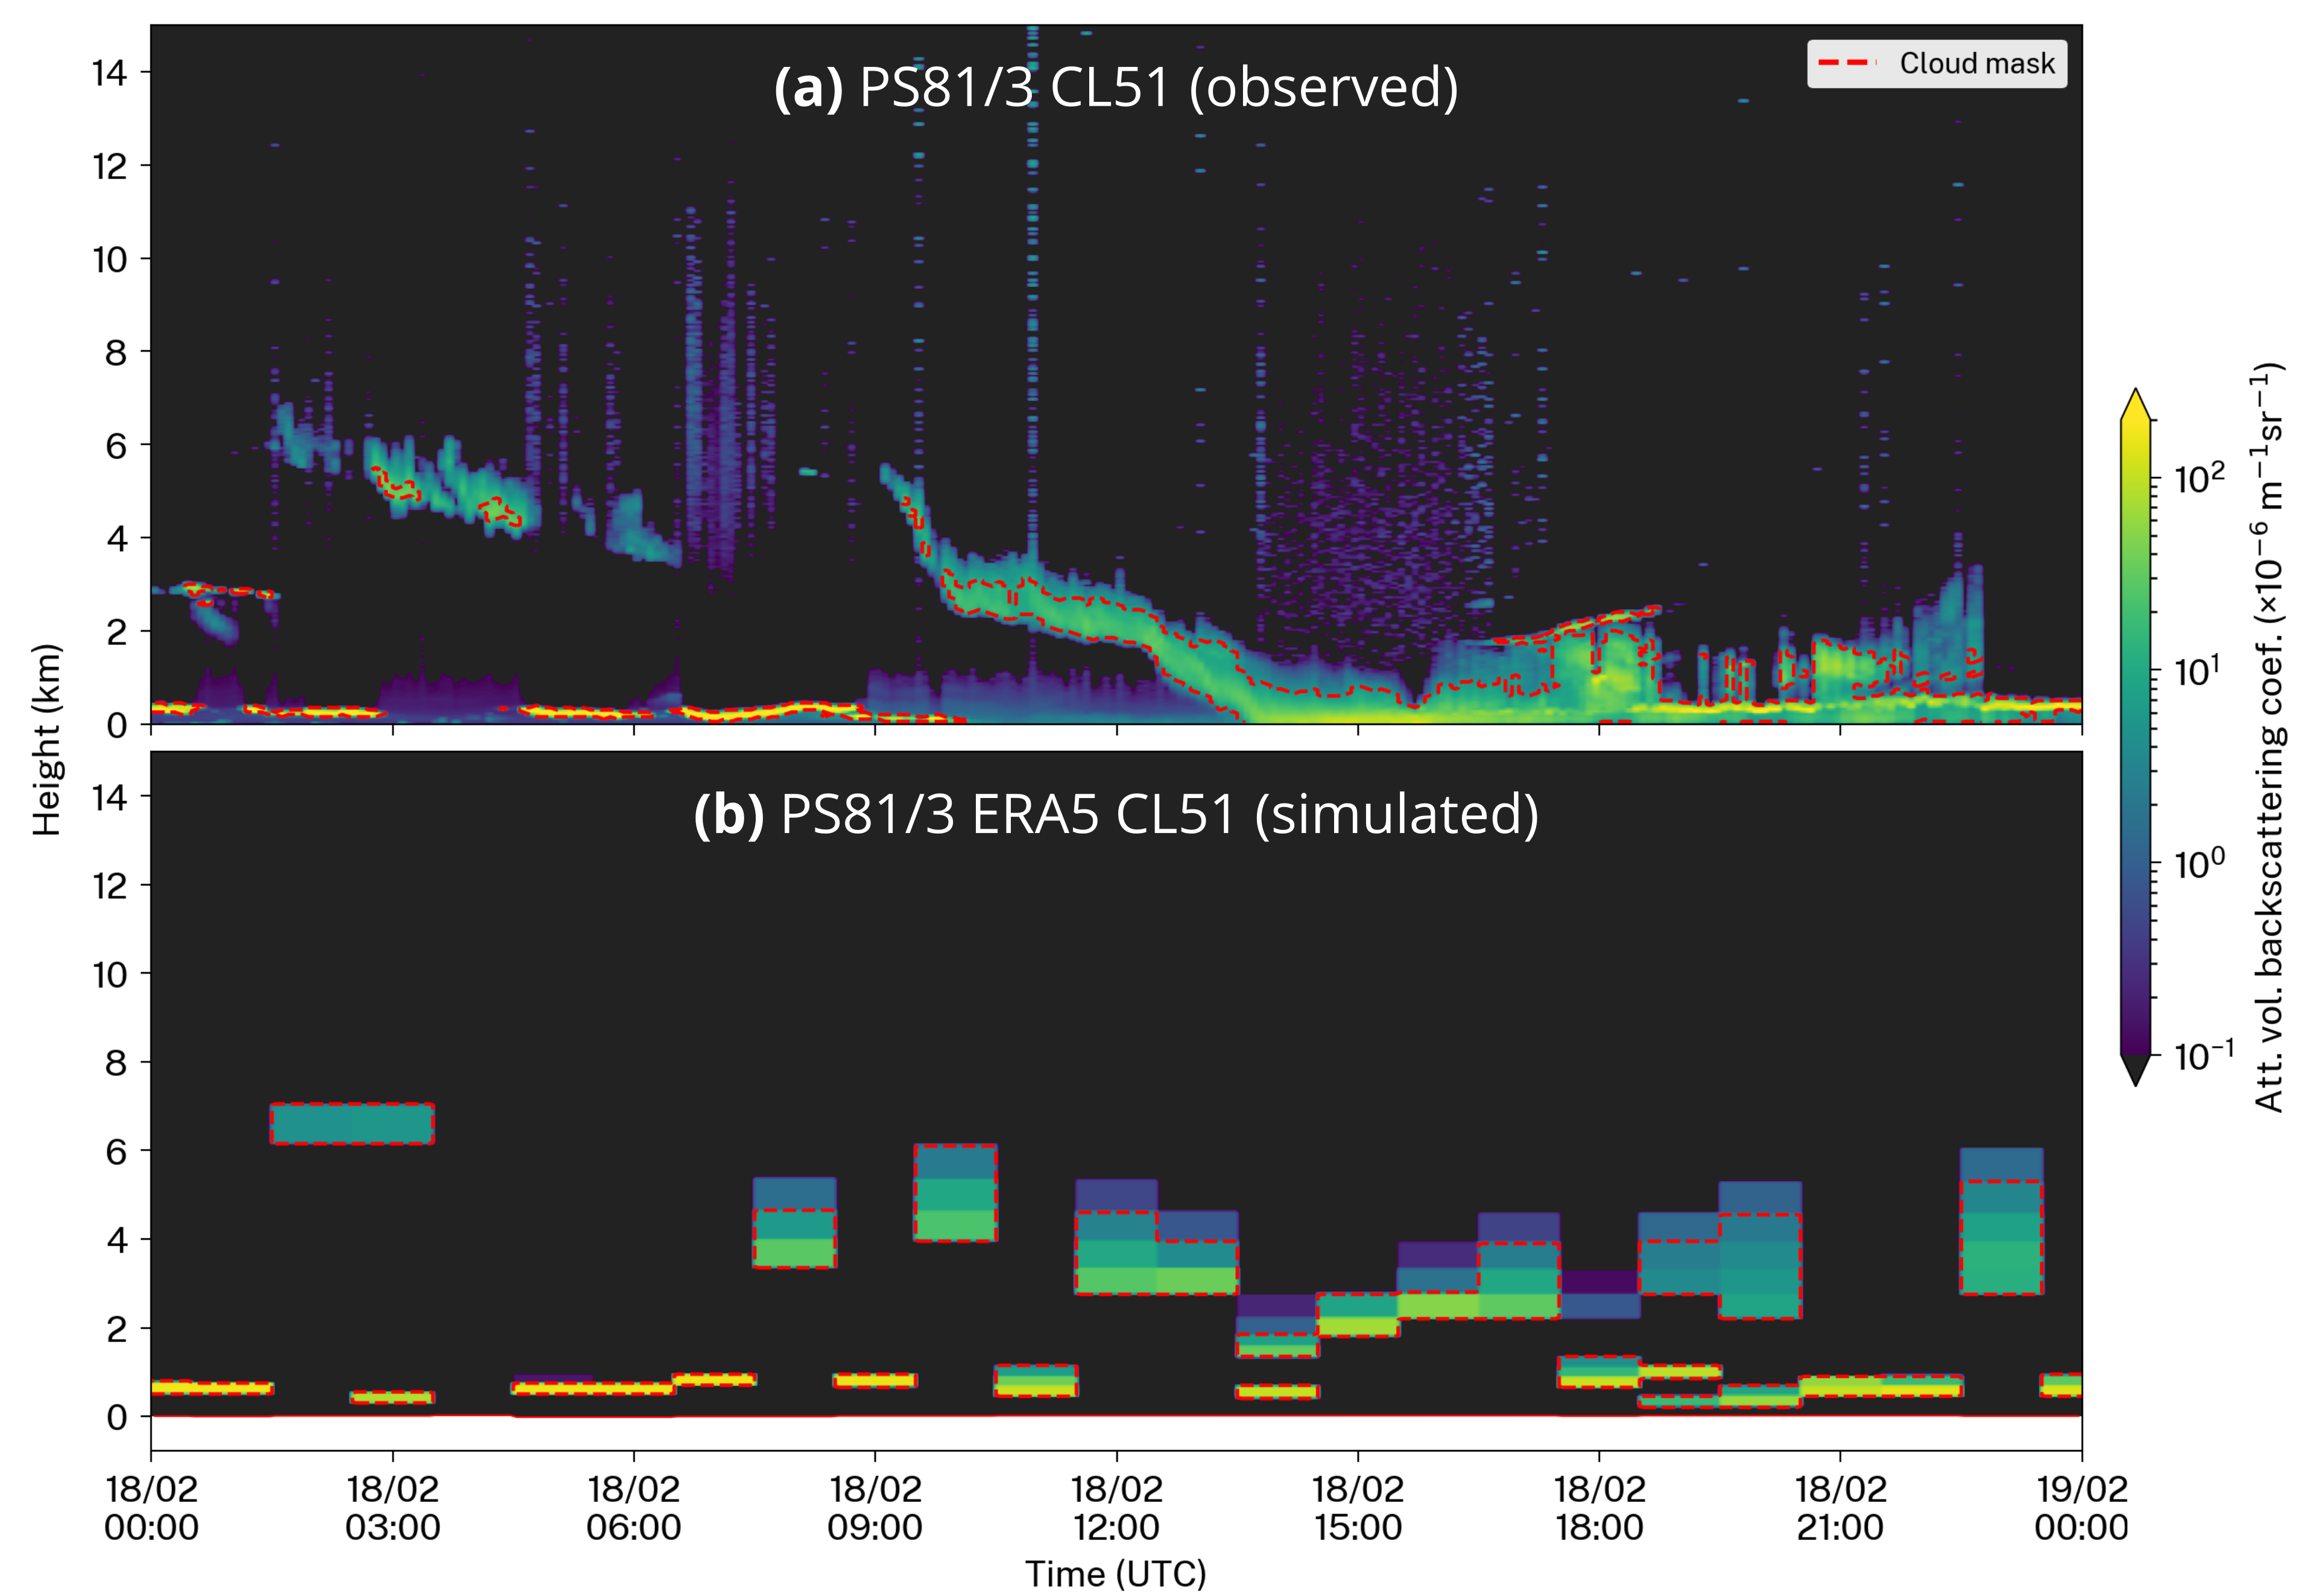
\includegraphics[width=\textwidth]{img/example.png}
\caption{
An example of the attenuated volume backscattering coefficient (AVBC) \textbf{(a)} measured by CL51 during 24~hours on the PS81/3 voyage and \textbf{(b)} an equivalent AVBC simulated with the ALCF from ERA5 data during the same time period. The red line identifies the cloud mask determined by the ALCF.
}
\label{fig:example}
\end{figure}

\subsection{Lufft CHM~15k}
\label{sec:chm15k}

The Lufft CHM~15k (photo in Fig.~\ref{fig:map}c) is a ceilometer operating at a near-infrared wavelength of 1064~nm. The maximum range is 15.4~km; the vertical resolution is 5~m in the near range (up to 150~m) and 15~m above; the sampling (temporal) resolution is 2~s; and the number of vertical levels is 1024. NetCDF files containing uncalibrated backscatter produced by the instrument were processed with the ALCF (Section~\ref{sec:alcf}) to again produce AVBC, cloud mask, cloud occurrence by height, and the total cloud fraction. The CHM~15k was used on four voyages (HMNZSW16, TAN1702, TAN1802, and NBP1704).

\subsection{ALCF}
\label{sec:alcf}

The Automatic Lidar and Ceilometer Framework (ALCF) is a ground-based lidar simulator and a tool for processing observed lidar data, supporting various instruments and models \cite{kuma2021}. It performs radiative transfer calculations to derive equivalent lidar AVBC in an atmospheric model, which can then be compared with observed AVBC. For this purpose, it takes the cloud fraction, liquid and ice mass mixing ratio, temperature, and pressure model fields as an input and is run offline (on the model output rather than inside the model code). The lidar simulator in the ALCF is based on the instrument simulator Cloud Feedback Model Intercomparison Project (CFMIP) Observation Simulator Package (COSP) \cite{bodas-salcedo2011}. After AVBC is calculated, a cloud mask, cloud occurrence by height, and the total cloud fraction are determined. The ALCF has been used by several research teams for model and reanalysis evaluation \cite{kuma2020,kremser2021,guyot2022,pei2023,whitehead2023,mcdonald2024}.

Absolute calibration of the observed backscatter was performed by comparing the measured clear-sky molecular backscatter statistically with simulated clear-sky molecular backscatter. AVBC was resampled to 5 min temporal resolution and 50~m vertical resolution to increase the signal-to-noise ratio while having enough resolution to detect small-scale cloud variability. The noise standard deviation was calculated from AVBC at the highest range, where no clouds are expected. A cloud mask was calculated from AVBC using a fixed threshold of $\mathrm{2\times 10^{-6} m^{-1}sr^{-1}}$ after subtracting 5 standard deviations of range-scaled noise. Fig.~\ref{fig:example}b shows an example of simulated Vaisala CL51 backscatter from ERA5 data, corresponding to a day of measurements by the instrument on the PS81/3 voyage.

\subsection{ICON}
\label{sec:icon}

A coupled (atmosphere--ocean) GSRM version of the ICON model is in development at the nextGEMS project \cite{hohenegger2023}. ICON is an exceptionally versatile model, allowing for simulations ranging from coarse-resolution ESM simulations, GSRM simulations, limited area model simulations, to large eddy simulations (LES), for both weather prediction and climate projections. ICON uses the atmospheric component ICON-A \cite{giorgetta2018}, whose physics is derived from ECHAM6 \cite{stevens2013}, and the ocean component ICON-O \cite{korn2022}. Earlier runs of the GSRM ICON from DYAMOND were evaluated by \citeA{mauritsen2022}.

Here, we use a free-running (i.e., the weather situation in the model does not correspond to reality) coupled GSRM simulation made for the purpose of climate projection. nextGEMS has so far produced four cycles of model runs. We used a Cycle 3 run \emph{ngc3028} produced in 2023 \cite{nextgems2023a,nextgems2023b} for a model time period of 20 January 2020 to 22 July 2025, of which we analyzed the period 2021--2024 (inclusive). While a Cycle 4 run was available, we could not use it due to a lack of availability of the necessary variables. The horizontal resolution of ngc3028 is about 5 km. The model output is available on 90 vertical levels and 3-hourly instantaneous temporal resolution.

Unlike current general circulation models (GCMs), the storm-resolving version of ICON does not use convective and cloud parameterization but relies on explicit simulation of convection and clouds on the model grid. Subgrid-scale clouds are not resolved, and the grid cell cloud fraction is always either 0 or 100\%. While this makes the code development simpler without having to rely on uncertain parameterizations, it can miss smaller-scale clouds below the grid resolution. Turbulence and cloud microphysics are still parameterized in this model, and aerosols are taken from a climatology. To account for the radiative effects of subgrid-scale clouds, a cloud inhomogeneity factor is introduced in the model, which scales down the cloud liquid water for radiative calculations. It ranges from 0.4 at lower tropospheric stability (LTS) of 0~K to 0.8 at 30~K. In addition, vertical mixing is enhanced in unstable and humid lower-tropospheric conditions, which reduces the amount of shallow clouds.

Because the analyzed ICON simulation was free-running (years 2021--2024, inclusive), weather and climate oscillations (such as the El Niño--Southern Oscillation) are not expected to be equivalent to reality at the same time and place. To compare with the observations collected during a different time period (years 2010--2021, inclusive), we compared the model output with observations at the same time of year and geographical location, as determined for each data point, such as a lidar profile or a radiosonde launch. In the ALCF, this was done using the \emph{override\_year} option (\url{https://alcf.peterkuma.net/documentation/cli/cmd_model.html}). For radiosonde profiles, the same mapping of time from was done. That is, when selecting an equivalent profile from the model, the time of the profile was changed so that the time relative to the start of the year was preserved, but the year was changed to one of the four years available in the model data. Thus, for every radiosonde launch, there were four equivalent model profiles. The geographical location was kept the same. We discuss briefly the implications of comparing the observations with a free-running model in Section~\ref{sec:limitations}.

\subsection{MERRA-2}

The Modern-Era Retrospective analysis for Research and Applications, Version 2 (MERRA-2) is a reanalysis produced by the Global Modeling and Assimilation Office at the NASA Goddard Space Flight Center \cite{gelaro2017}. It uses version 5.12.4 of the Goddard Earth Observing System (GEOS) atmospheric model \cite{rienecker2008,molod2015}. Non-convective clouds (condensation, autoconversion, and evaporation) are parameterized using a prognostic scheme \cite{bacmeister2006}, and sub-grid cloud fraction is determined using total water distribution and a critical relative humidity threshold. The reanalysis output analyzed here is available at a spatial resolution of 0.5° of latitude and 0.625° of longitude, which is about 56 km in the North--South direction and 35 km in the East--West direction at 60°S. The number of vertical model levels is 72. Here, we use the following products: 1-hourly instantaneous 2D single-level diagnostics (M2I1NXASM) for 2-m temperature and humidity; 3-hourly instantaneous 3D assimilated meteorological fields (M2I3NVASM) for cloud quantities, pressure, and temperature; 1-hourly average 2D surface flux diagnostics (M2T1NXFLX) for precipitation; and 1-hourly average 2D radiation diagnostics (M2T1NXRAD) for radiation quantities \cite{merra2}.

\subsection{ERA5}

ERA5 \cite{era5} is a reanalysis produced by the ECMWF. It is based on a numerical weather prediction model IFS version CY41R2. It uses the \citeA{tiedtke1993} prognostic cloud scheme and \citeA{forbes2014} for mixed-phase clouds. The horizontal resolution is 0.25° in latitude and longitude, which is about 28~km in the North--South direction and 14~km in the East--West direction at 60°S. Internally, the model uses 137 vertical levels. Here, we use output at 1-hourly instantaneous time intervals, except for radiation quantities, which are accumulations (from these we calculate daily means). Vertically resolved quantities are made available on 37 pressure levels.

\subsection{CERES}

TOA radiation quantities are taken from the CERES instruments onboard the Terra and Aqua satellites \cite{wielicki1996,loeb2018}. In our analysis, we used the adjusted all-sky SW and LW upwelling fluxes at TOA from the synoptic TOA and surface fluxes and clouds 1-degree daily edition 4A product (CER\_SYN1deg-Day\_Terra-Aqua-MODIS\_Edition4A) \cite{doelling2013,doelling2016}.

Radiation calculations presented in the results (Section~\ref{sec:results}) were completed such that they always represent daily means in order to be consistent with the CERES SYN1deg data. Therefore, every instantaneous profile in the simulated lidar data was assigned a daily mean radiation value corresponding to the day (in the Coordinated Universal Time; UTC). In turn, the average radiation during the entire voyage or station observation period was calculated as the average of the profile values. In the observed lidar data, the daily mean radiation value was taken from the spatially and temporally co-located CERES SYN1deg data for the day (in UTC). The voyage or station average was calculated in the same way.

\begin{figure}[b!]
\centering
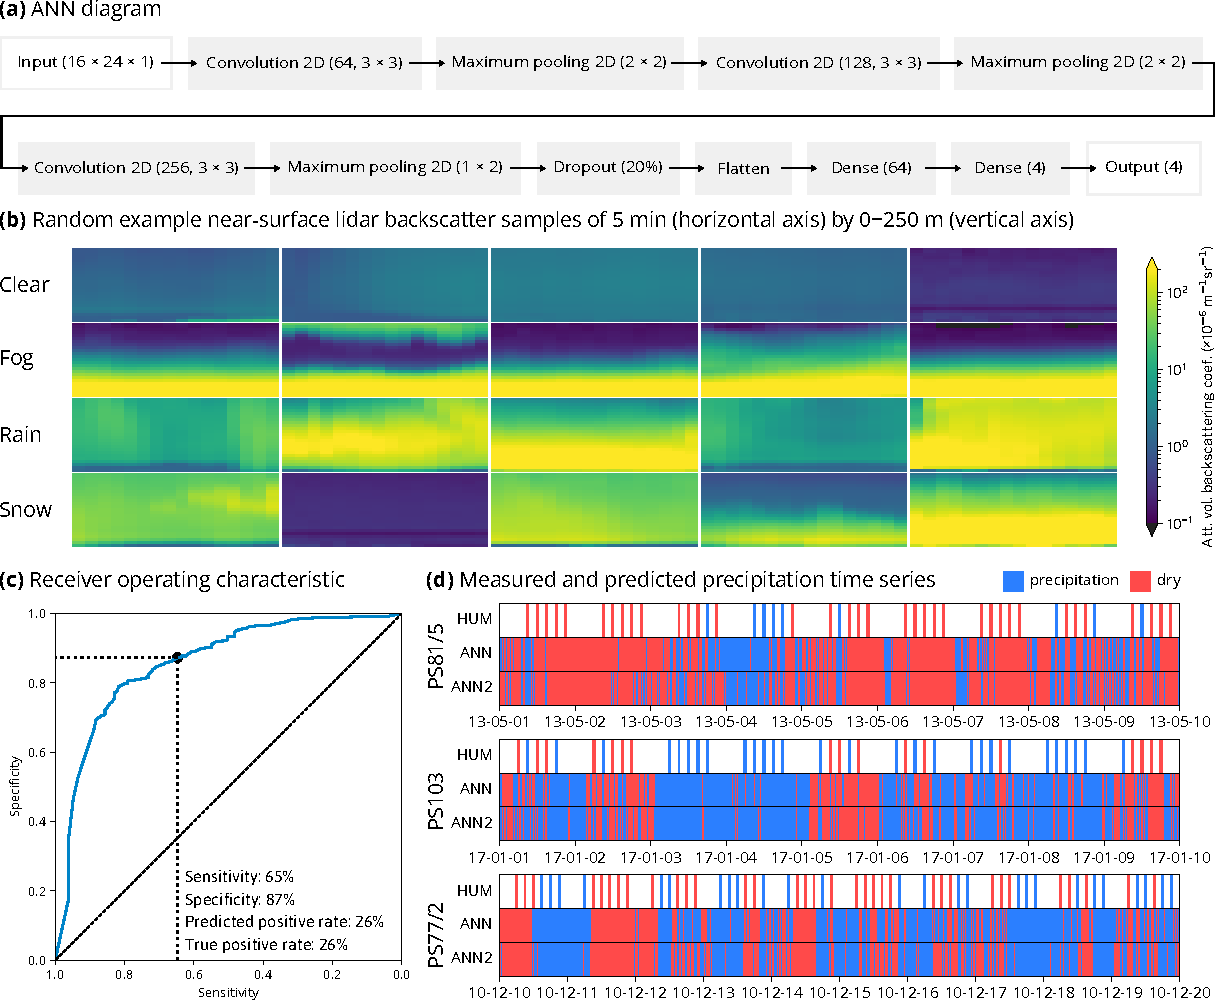
\includegraphics[width=\textwidth]{img/ann.pdf}
\caption{
Artificial neural network (ANN) for prediction of precipitation in lidar backscatter. \textbf{(a)} Diagram showing the TensorFlow structure of the ANN, \textbf{(b)} randomly selected example samples of near-surface backscatter in four categories (clear, fog, rain, and snow), as determined by coincident human-performed weather observations, \textbf{(c)} receiver operating characteristic diagram of the ANN, \textbf{(d)} examples of 10-day time series of human-observed (``HUM'') and predicted precipitation based on an ANN trained on all voyages (``ANN'') and all voyages except for the shown voyage (``ANN2'') during three randomly selected voyages with the available data. Here, by ``randomly selected,'' we mean selected from the top of a permutation generated by a pseudo-random number generator to prevent authors' bias in the selection.
}
\label{fig:ann}
\end{figure}

\subsection{Precipitation Identification Using Machine Learning}
\label{sec:ann}

Precipitation can cause strong enough lidar backscattering to be recognized as clouds by the threshold-based cloud detection method used in the ALCF. This is undesirable if equivalent precipitation backscatter is not included in the simulated lidar profiles. It was not possible to include precipitation simulation in the ALCF due to the absence of required fields in the ICON model output and the reanalysis data (the liquid and ice precipitation mass mixing ratios). The required radiation calculations for precipitation are also currently not implemented in the ALCF, even though this is a planned future addition. In order to achieve a fair comparison of observations with model output, we exclude observed and simulated lidar profiles with precipitation, either manually or using an automated method. It is relatively difficult to distinguish precipitation backscatter from cloud backscatter in lidar observations, especially when only one wavelength channel and no polarized channel are available. In models, the same can be accomplished relatively easily by excluding profiles exceeding a certain surface precipitation flux. In the observations, using precipitation flux measurements from rain gauges can be very unreliable on ships due to ship movement, turbulence caused by nearby ship structures, and sea spray. Our analysis of rain gauge data from the RV \emph{Tangaroa} showed large discrepancies between the rain gauge time series and human-performed synoptic observations, as well as large inconsistencies in the rain gauge time series. Human-performed observations of precipitation presence or absence are expected to be reliable but only cover a limited set of times. Therefore, it was desirable to implement a method of detecting precipitation from observed backscatter profiles alone.

On the RV \emph{Polarstern} voyages, regular human-performed synoptic observations were available and included precipitation presence or absence and type. We used this dataset to train a convolutional artificial neural network (ANN) to recognize profiles with precipitation from lidar backscatter (Fig.~\ref{fig:ann}a), implemented in the TensorFlow ANN framework \cite{tensorflow}. Samples of short time intervals (10~min) of near-surface lidar backscatter (0–250 m) were classified as clear, rain, snow, and fog, using the synoptic observations as a training dataset (Fig.~\ref{fig:ann}b). From these, a binary, mutually exclusive classification of profiles as precipitating (rain or snow) or dry (clear or fog) was derived. For detecting model and reanalysis precipitation, we used a fixed threshold for surface precipitation flux of 0.1 mm h$^{-1}$ (the ANN was not used).

The ANN achieved 65\% sensitivity and 87\% specificity when the true positive rate (26\%) was made to match observations. The receiver operating characteristic curve is shown in Fig.~\ref{fig:ann}c. We considered these rates satisfactory for the purpose of filtering precipitation profiles. Fig.~\ref{fig:ann}d shows examples of the predicted precipitation compared to human-performed observations. The main ANN (`ANN` in Fig.~\ref{fig:ann}) was trained on all data, and ancillary ANNs (`ANN2` in Fig.~\ref{fig:ann}) were trained on all data except for each voyage. These were used for testing the results relative to each voyage.

\begin{figure}[b!]
\centering
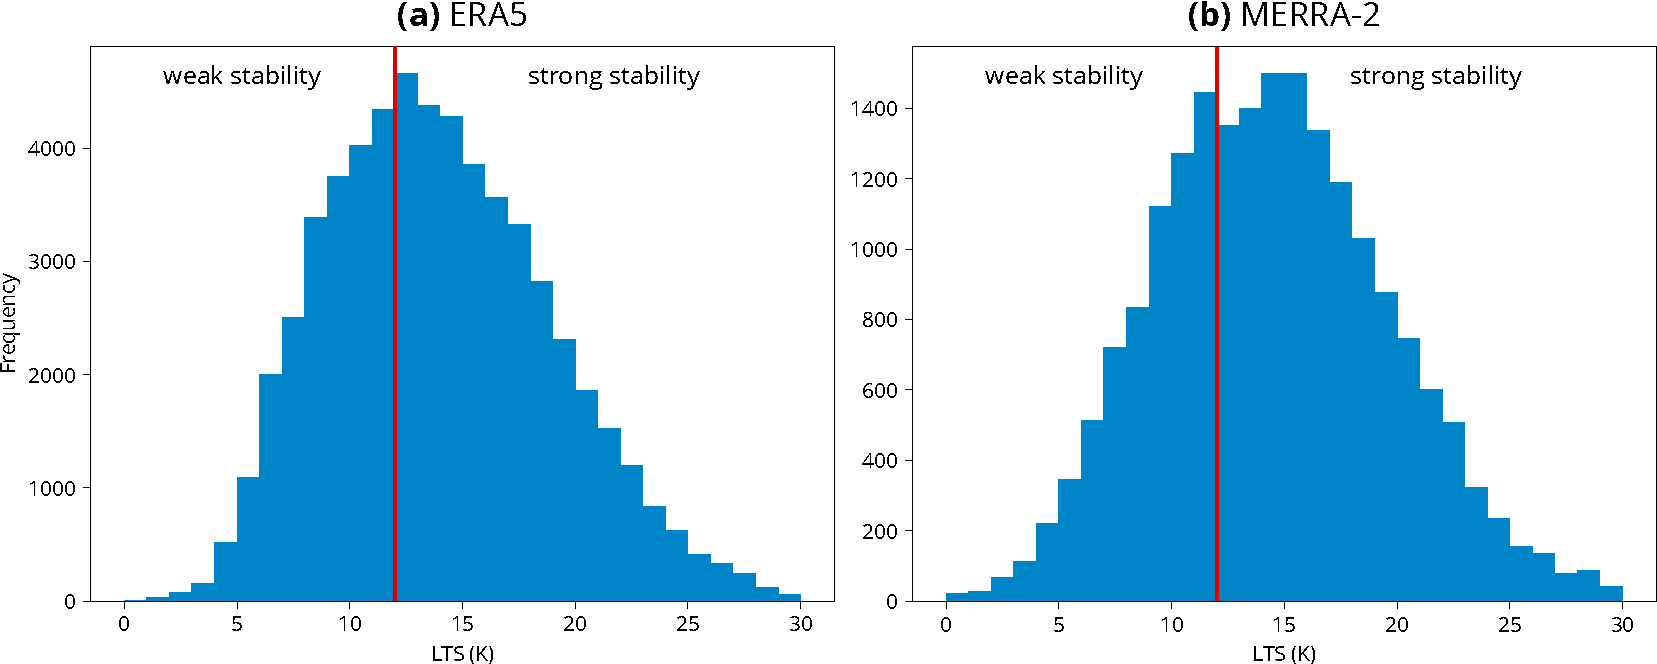
\includegraphics[width=\textwidth]{img/lts_dist.pdf}
\caption{
Lower tropospheric stability (LTS) distribution in \textbf{(a)} ERA5 and \textbf{(b)} MERRA-2 calculated for the 31 voyage tracks and one station from the highest instantaneous temporal resolution data available. Shown is also the chosen dividing threshold of 12 K for conditions of weak and strong stability.
}
\label{fig:lts}
\end{figure}

\subsection{Partitioning by Cyclonic Activity and Stability}
\label{sec:cyclone-stability}

We partitioned our data into two mutually exclusive subsets by cyclonic activity. For this purpose, we used a cyclone tracking algorithm to identify extratropical and polar cyclones (ECs and PCs) over the SO in the reanalysis and ICON data. We used the open-source cyclone tracking package CyTRACK \cite{perez-alarcon2024}. Generally, what constitutes an EC is considered relatively arbitrary due to the very large variability of ECs \cite{neu2013}. We used the mean sea level pressure field and horizontal wind speed fields as input to the CyTRACK algorithm. The algorithm uses pressure and wind speed thresholds as well as tracking across time steps to identify cyclone centers and radii in each time step. With this information, we could classify geographical areas as either cyclonic or non-cyclonic. Due to a relatively small total area covered by cyclones (as identified by the cyclone center and radius), we chose a circle of a double radius (relative to one identified by CyTRACK) centered at the cyclone center as a cyclonic area for every time step and cyclone. All other areas were identified as non-cyclonic. For identifying cyclones in the observations and the reanalyses, ERA5 pressure and wind fields were used as the input to CyTRACK. This is justified by the fact that the large-scale pressure and wind fields in ERA5 are likely sufficiently close to reality. \citeA{mcerlich2023} have shown that wind is simulated well in ERA5 relative to the WindSat polarimetric microwave radiometer measurements \cite{meissner2009}. For identifying cyclones in ICON, its own pressure and wind fields were used as the input to CyTRACK, because the model is free-running, and thus the pressure and wind fields are different from reality. Subsetting by proximity to cyclones is a relatively crude measure because it does not take into account the different sectors of cyclones, which are commonly associated with different weather situations. However, this was a choice made for simplicity of the analysis, given the amount of data.

In addition to the above, we partitioned our data into two mutually exclusive subsets based on LTS, which is derived as the difference between the potential temperature at 700~hPa and the surface. Based on a histogram of LTS in ERA5 and MERRA-2 calculated at all voyage tracks and stations (Fig.~\ref{fig:lts}), we determined a statistically-based dividing threshold of 12~K for weak stability ($<$~12~K) and strong stability ($\geq$~12~K) conditions.

\section{Results}
\label{sec:results}

\begin{figure}[p!]
\centering
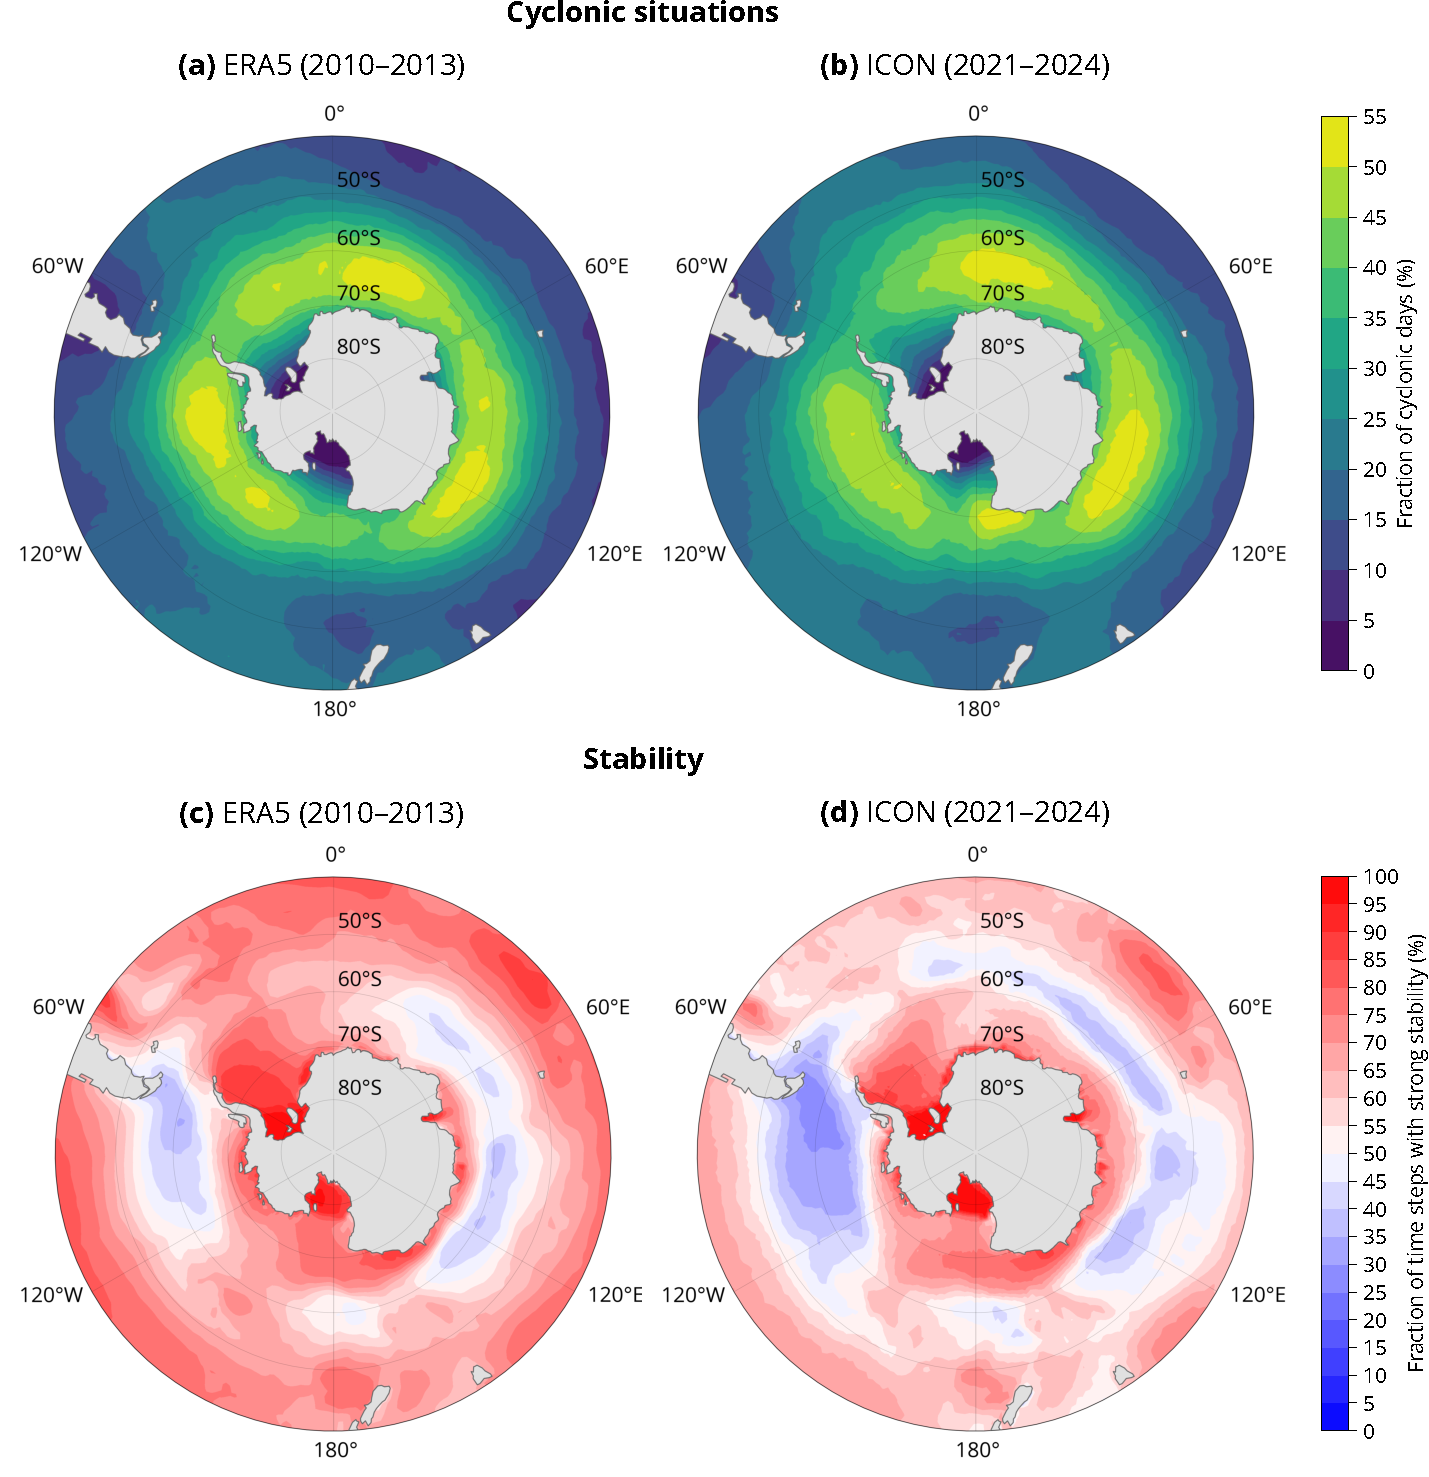
\includegraphics[width=\textwidth]{img/cyc_stab_dist.pdf}
\caption{
Geographical distribution of \textbf{(a, b)} cyclonic days and \textbf{(b, d)} strong stability (LTS~$\geq$~12~K) time steps in \textbf{(a, c)} ERA5 in years 2010--2013 (inclusive) and \textbf{(b, d)} ICON in model years 2021--2023 (free running). Cyclonic days are expressed as a fraction of the number of days with cyclonic activity, defined as grid points located within a double radius of any cyclone on a given day (UTC), as identified by CyTRACK.
}
\label{fig:cyclone-stability}
\end{figure}

\subsection{Cyclonic Activity and Stability}

Fig.~\ref{fig:cyclone-stability}a, b show a geographical distribution of the fraction of cyclonic days as determined by the cyclone tracking algorithm applied to the ERA5 reanalysis and ICON data (Section~\ref{sec:cyclone-stability}). As expected, the strongest cyclonic activity is in the high-latitude SO zone, and it is relatively zonally symmetric at all latitudes. The pattern matches reasonably well with \citeA{hoskins2005}. While both reanalysis and the model agree within about 8\% in most areas, ICON is prevailingly more cyclonic by about 4\%. There are clear differences, particularly in the highest occurrence rate regions, such as around Cape Adare, which is by up to 20\% more cyclonic in ICON, and the Weddell and Bellingshausen Seas, where ICON is less cyclonic by up to 10\%. These differences might, however, stem from the relatively short time periods of comparison (4 years) and the fact that the model is free-running.

Fig.~\ref{fig:cyclone-stability}c, d show a geographical distribution of the conditions of weak and strong stability as determined by the LTS (Section~\ref{sec:cyclone-stability}). Conditions of weak stability are prevalent in the mid-to-high SO (with respect to our SO partitioning; 50--65°S), which might be explained by the relatively cold near-surface air overlying the relatively warm sea surface. Conditions of strong stability are prevalent elsewhere over the SO. The distribution is also less zonally symmetric than the cyclonic activity. In the high-latitude SO, the presence of sea ice might have a substantial stabilizing effect \cite{knight2024}. The ERA5 reanalysis is also substantially more stable than ICON across the whole region.

\begin{figure}[p!]
\centerline{
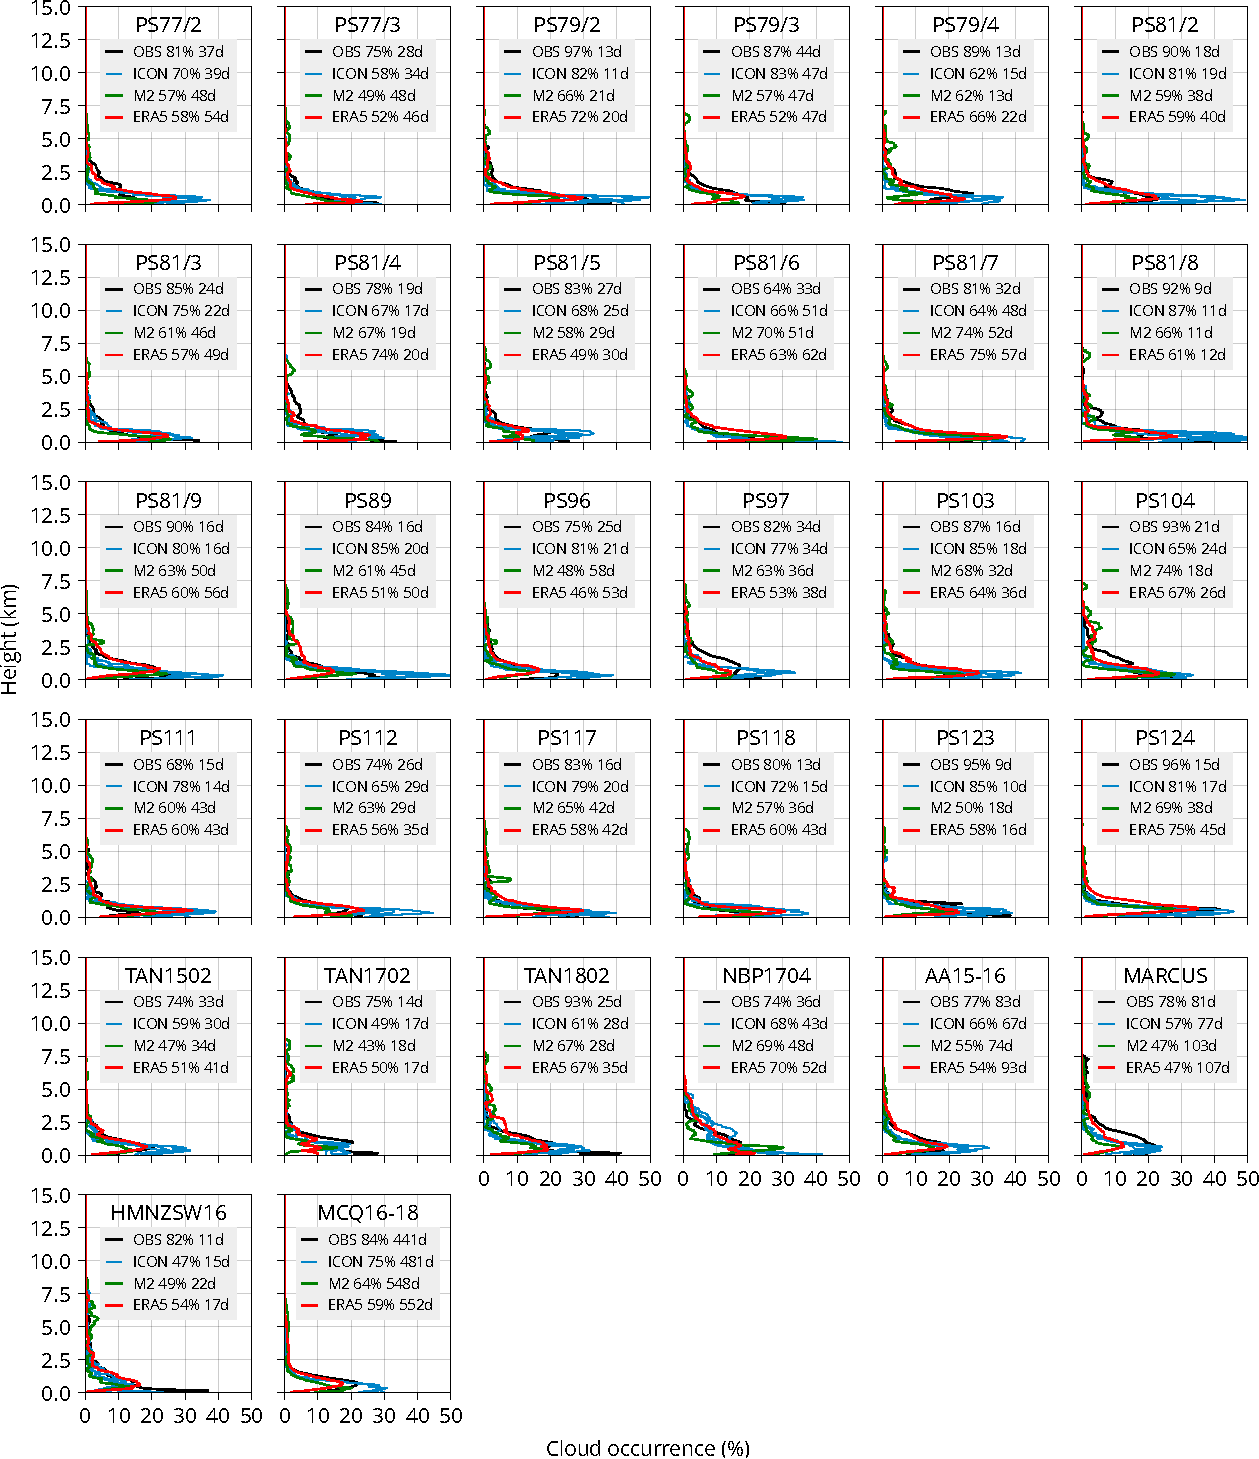
\includegraphics[width=1.06\textwidth]{img/cloud_occurrence_panel.pdf}
}
\caption{
Cloud occurrence by height for the 31 voyages and one sub-Antarctic station (MICRE) in observations (O) and simulated by the ALCF from the ICON model (I), MERRA‐2 (M), and ERA5 reanalysis data (E). The numbers in the legend indicate the total cloud fraction and the number of days of data. Multiple lines of ICON profiles are for each of the four years of model data available.
}
\label{fig:cloud-occurrence-panel}
\end{figure}

\subsection{Cloud Occurrence by Height}
\label{sec:cloud-occurrence}

We used the ALCF to derive cloud occurrence by height and the total cloud fraction from observations, ICON, ERA5, and MERRA-2. The results for all campaigns individually are shown in Fig.~\ref{fig:cloud-occurrence-panel}. In addition, we aggregated the campaigns by calculating the averages and percentiles of all individual profiles, presented in Fig.~\ref{fig:cloud-occurrence}. The analysis shows that the total cloud fraction (determined as the fraction of profiles with clouds at any height in the lidar cloud mask) is underestimated in ICON by about 10\% and in the reanalyses by about 20\%. When analyzed by height, ICON overestimates cloud occurrence below 1 km and underestimates it above; MERRA-2 underestimates cloud occurrence at all heights by up to about 10\%, especially near the surface; and ERA5 simulates cloud occurrence relatively well above 1 km but strongly underestimates it near the surface. We note that fog or near-surface clouds are strongly underestimated in the reanalyses (fog and clouds are both included in the cloud occurrence). As shown in Fig.~\ref{fig:cloud-occurrence-panel}, the biases are relatively consistent across the campaigns and longitudes. We conclude that the ICON results the observations better than the reanalyses in this metric.

For all observations considered (Fig.~\ref{fig:cloud-occurrence}a), the data show cloud occurrence peaking nearly at the surface, whereas the models show a higher peak (at about 500~m). The models generally underestimate the total cloud fraction by 10--20\% and show a strong reduction in cloud occurrence near the surface, which is not supported by the observations. ICON and ERA5 overestimate cloud occurrence at their peak (between 0--1~km). Above 1~km, ICON and MERRA-2 underestimate cloud occurrence, but ERA5 is accurate to about 3\% or less. The exaggerated peak in models is partly supported by the lifting condensation level (LCL) distribution, which peaks higher by about 200~m in the models than in the observations (nearly at the surface), although this is not very pronounced. This is indicative of near-surface relative humidity being often close to saturation in the observations but not in the models.

When subsetted by latitude (Fig.~\ref{fig:cloud-occurrence}b, c), we see that the low-latitude SO zone displays a stronger peak of cloud occurrence near the surface than the high-latitude SO zone, and this could be because higher latitudes have less stable atmospheric profiles. The low- and high-latitude SO zones show similar biases in models as in the general case, but ERA5 does not overestimate the peak in the low-latitude SO zone (near-surface cloud occurrence is still strongly underestimated).

When subsetted by cyclonic and non-cyclonic situations (Fig.~\ref{fig:cloud-occurrence}d, e), we see that the cyclonic situations have a larger amount of observed cloudiness, including peak and total cloud fraction, both by about 7\%. In the cyclonic situations, the model vertical profiles of cloud occurrence compare well with observations, but they peak higher by about 200 m and stronger by about 8\%. The reanalyses still tend to underestimate cloud occurrence above 1 km by about 5\% and near the surface by about 14\%. Non-cyclonic situations are similar to the general case, partially also because they form the majority of cases.

When subsetted by conditions of weak and strong stability (Fig.~\ref{fig:cloud-occurrence}f, g), as defined in Section~\ref{sec:cyclone-stability}, we see that in situations of strong stability, cloud occurrence peaks strongly nearly at the surface in observations, compared to situations of weak stability, where the peak is more diffuse between 0 and 1~km. It is worth mentioning that conditions of strong stability might be associated with the formation of advection fog, such as in situations of warm air advection from the north over a colder sea surface, thus inducing fog formation by cooling of the warm and humid air by the cold surface. In situations of strong stability, the models have smaller biases than in weak stability, with an overestimated peak by up to 12\%, underestimated cloud occurrence above 1~km by up to 5\%, and underestimated cloud occurrence near the surface by about 11\%. In situations of weak stability, the bias in ICON is very pronounced, with a much stronger peak at about 500~m; ERA5 underestimates cloud occurrence below 1~km (especially near the surface); and MERRA-2 underestimates cloud occurrence even more strongly.

In all situations, even when the models overestimate cloud occurrence at some altitudes, they always substantially underestimate the total cloud fraction. ICON can be generally characterized as substantially overestimating cloud occurrence below 1 km and underestimating above, underestimating the total cloud fraction, and showing the greatest biases in conditions of weak stability and non-cyclonic conditions. It also shows a peak of cloud occurrence at higher altitudes than observations (500~m vs. near the surface), and correspondingly, its LCL tends to be higher. MERRA-2 can be generally characterized as underestimating cloud occurrence at nearly all altitudes as well as the total cloud fraction, but mostly above and below 500~m (the peak at 500~m is well represented). MERRA-2 displays the largest errors relative to observations in the low-latitude SO zone and in situations of weak stability. ERA5 can be generally characterized as representing cloud occurrence correctly above about 1--1.5~km, overestimating below, but underestimating near-surface cloud occurrence (0--500~m). The total cloud fraction is strongly underestimated in all situations. ERA5 has a tendency towards underestimation in the low-latitude SO zone and situations of weak stability; conversely, it overestimates in the high-latitude SO zone and conditions of strong stability.

\begin{figure}[p!]
\centering
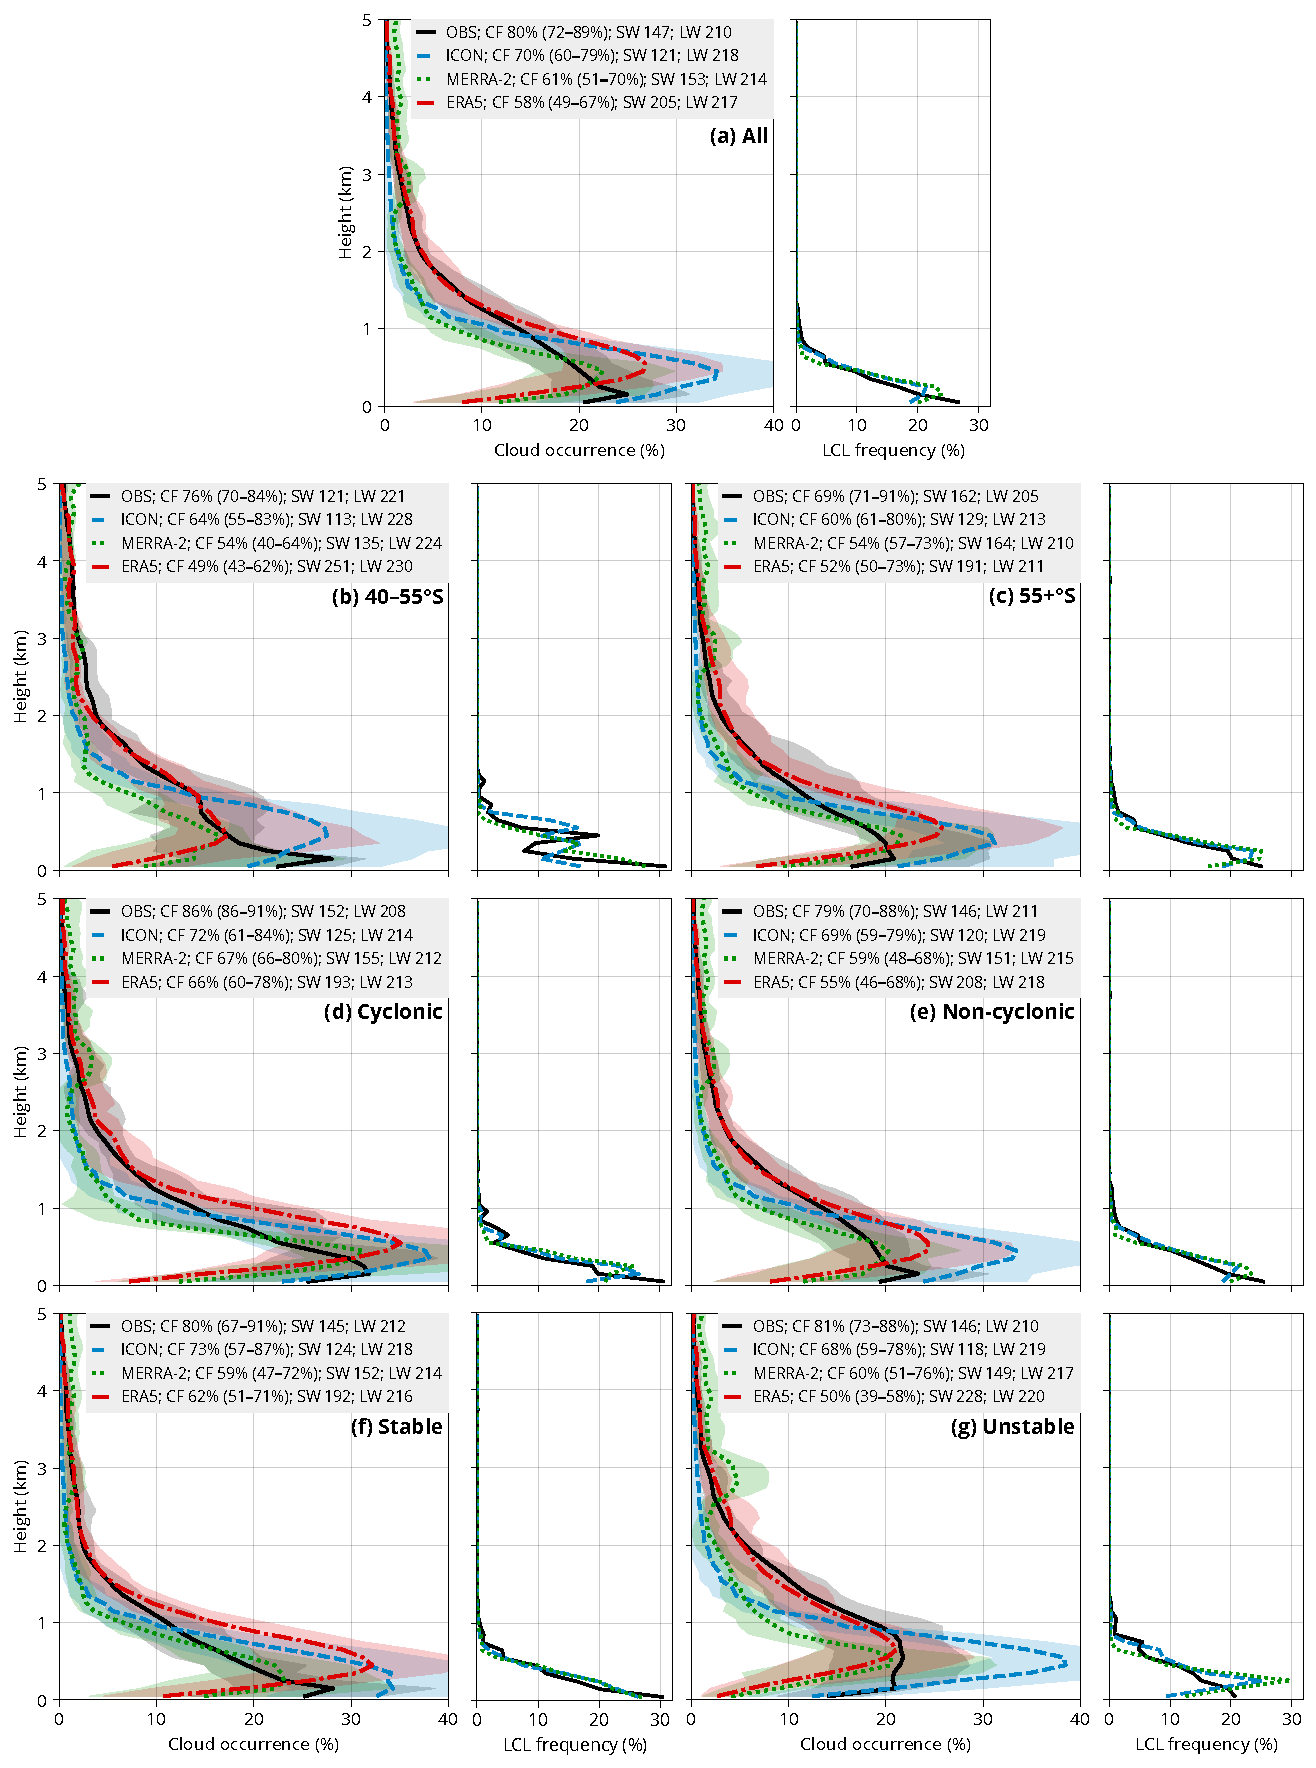
\includegraphics[width=\textwidth]{img/cl_agg.pdf}
\caption{
Cloud occurrence by height calculated as the average of all voyages and stations and lifting condensation level (LCL) distribution. The LCL is derived from radiosonde profiles and equivalent model profiles, which were not available for all voyages and times. The total cloud fraction (CF), average shortwave (SW), and longwave (LW) and the relative frequency of occurrence (RFO) are shown. The bands are the 16$^\mathrm{th}$--84$^\mathrm{th}$ percentile, calculated from the set of all voyages and stations.
}
\label{fig:cloud-occurrence}
\end{figure}

\subsection{Top of Atmosphere Radiation}

In Fig.~\ref{fig:cloud-occurrence}, we also show outgoing shortwave and longwave top of atmosphere radiation. In observations, these come from daily mean CERES measurements averaged over the voyage tracks or a station location, whereas in the models they come from daily means of TOA radiation in the model output averaged over the same location and time periods. In the free-running ICON model, the time period is mapped onto the available years, as explained in Section~\ref{sec:icon}.

In the general case (Fig.~\ref{fig:cloud-occurrence}a), ICON underestimates the outgoing SW radiation by 26 Wm$^{-2}$ and the reanalyses MERRA-2 and ERA5 are much closer but overestimate it by 6 and 14 Wm$^{-2}$, respectively. While in ICON, this is in line with the underestimated total cloud fraction by 10\%, in the reanalyses this is the opposite result as expected from the underestimated total cloud fraction by about 20\%. The likely explanation is an overestimated cloud albedo, compensating for the lack of cloud area.

In contrast, LW radiation is affected by much smaller biases than SW radiation, which is expected due to the prevailing low-level clouds having similar temperature as the surface. In ICON, the outgoing LW radiation is overestimated by 8\%, which could be caused by an underestimated total cloud fraction exposing a larger sea surface area to cooling to space, which is typically warmer than the atmospheric temperature at 0--2~km, where most of the clouds are located. In the MERRA-2 and ERA5 reanalyses, the LW biases are also slightly positive by 4 and 7~Wm$^{-2}$. This is again in line with the underestimated total cloud fraction by about 20\%. However, if the clouds are too thick, as expected from the SW results, this might also provide a compensating effect, in which too small a cloud area is counteracted by greater thermal emissivity, thus reducing the outgoing LW radiation more relative to thinner clouds. For thin clouds, the outgoing TOA LW radiation originates both from the warmer surface (partly blocked by the clouds) and the clouds, whereas for thick clouds, the outgoing TOA LW radiation originates mostly from the colder-than-surface clouds.

In all the subsets (Fig.~\ref{fig:cloud-occurrence}b--g), the same type of bias is present as in the general case -- the outgoing SW radiation is underestimated in ICON and overestimated in MERRA-2 and ERA5, and the outgoing LW radiation is overestimated in all the models. Even though the total cloud fraction is lower by 7\% over the high-latitude SO than the low-latitude SO, the outgoing SW radiation is much greater by 41~Wm$^{-2}$, implying a much greater cloud albedo over the high-latitude SO. ICON has the same contrast between these two regions in the total cloud fraction and SW radiation, but the outgoing SW radiation difference between the regions is much smaller (16~Wm$^{-2}$). The reanalyses do not show this type of contrast between the regions. The physical reason for this might be that the prevalence of fog or low-level clouds over the low-latitude SO and their relative lack over the high-latitude SO in observations is not reproduced in the models (Fig.~\ref{fig:cloud-occurrence}b--c).

\subsection{Cloud Cover}
\label{sec:cloud-cover}

We also analyzed the daily cloud cover (total cloud fraction) distribution. This is a measure of cloudiness, irrespective of height, calculated over the course of a day (UTC). A cloud detected at any height means that the lidar profile was classified as cloudy; otherwise, it was classified as a clear sky. When all profiles in a day are taken together, the cloud cover for the day is defined as the fraction of cloudy profiles in the total number of profiles, expressed in oktas (multiples of 1/8). The same calculation is done for the lidar observations as for the simulated lidar profiles. We use the term ``okta'' independently of its use in instantaneous synoptic observations, and here it simply means 1/8 (0.125\%) of the daily cloud cover.

In Fig.~\ref{fig:cloud-cover} we show the results for the same subsets of data as in Section~\ref{sec:cloud-occurrence}. Observations display the highest proportion of high cloud cover values (5--8~oktas), peaking at 7~oktas. This pattern is not represented by ICON or either reanalysis. While ICON is closest to matching the observed distribution, it tends to be 1~okta clearer than the observations, peaking at 6~oktas, and substantially underestimating days with 8~oktas. Overall, the reanalyses show results similar to each other, underestimating cloud cover by about 2~oktas and strongly underestimating days with 7 and 8~oktas. Of the two reanalyses, MERRA-2 has slightly higher cloud cover than ERA5, by about 6\% at 6 octas, which makes it more consistent with observations.

When analyzed by subsets, observations in the cyclonic subset show the highest cloud cover, with 8~oktas occurring on one half of such days (Fig.~\ref{fig:cloud-cover}d). This sensitivity to cyclonic conditions is not observed in ICON or the reanalyses. Interestingly, clear sky days (0~oktas) also have a local maximum peaking at about 15\% in this subset. When we contrast the low- and high-latitude zones, we see that the high-latitude zone tends to have greater cloud cover, peaking at 8~oktas (Fig.~\ref{fig:cloud-cover}c). The high-latitude zone also has almost no clear sky or small cloud cover cases (0--4~oktas). ICON and the reanalyses represent this characteristic of the distribution well for 0--3~oktas, but otherwise show biases similar to the general case. One of the greatest biases is present in ERA5 in the subset of weak stability, in which ERA5 peaks at 3~oktas, while the observations peak at 7~oktas and show negligible cloud cover below 5~oktas.

\begin{figure}[p!]
\centering
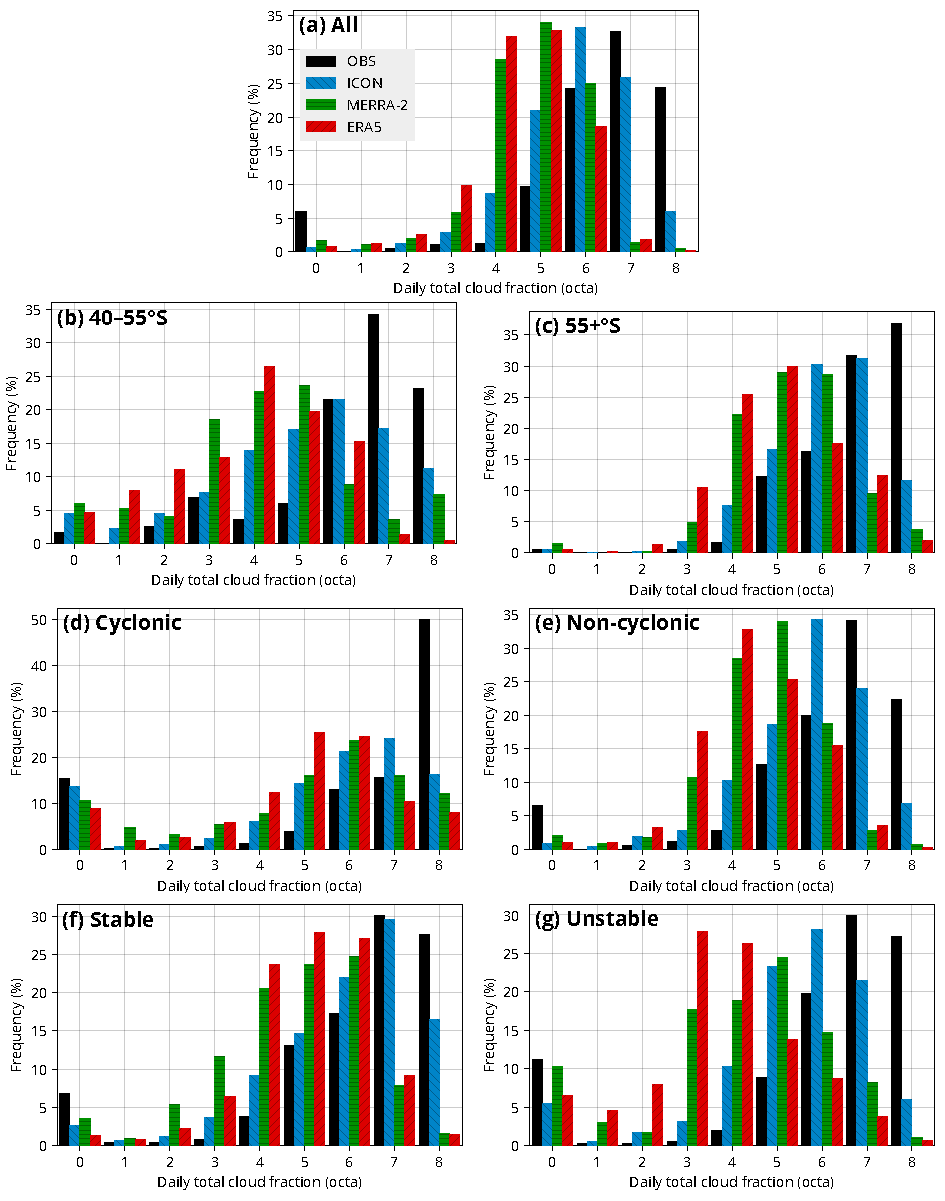
\includegraphics[width=\textwidth]{img/clt_hist.pdf}
\caption{
Daily total cloud fraction histograms calculated as the average of all voyage and station histograms. The total cloud fraction of a day (UTC) is calculated as a fraction of cloudy (based on the cloud mask) observed (OBS) or simulated lidar profiles. The models and subsets are as in Fig.~\ref{fig:cloud-occurrence}.
}
\label{fig:cloud-cover}
\end{figure}

\begin{figure}[p!]
\centering
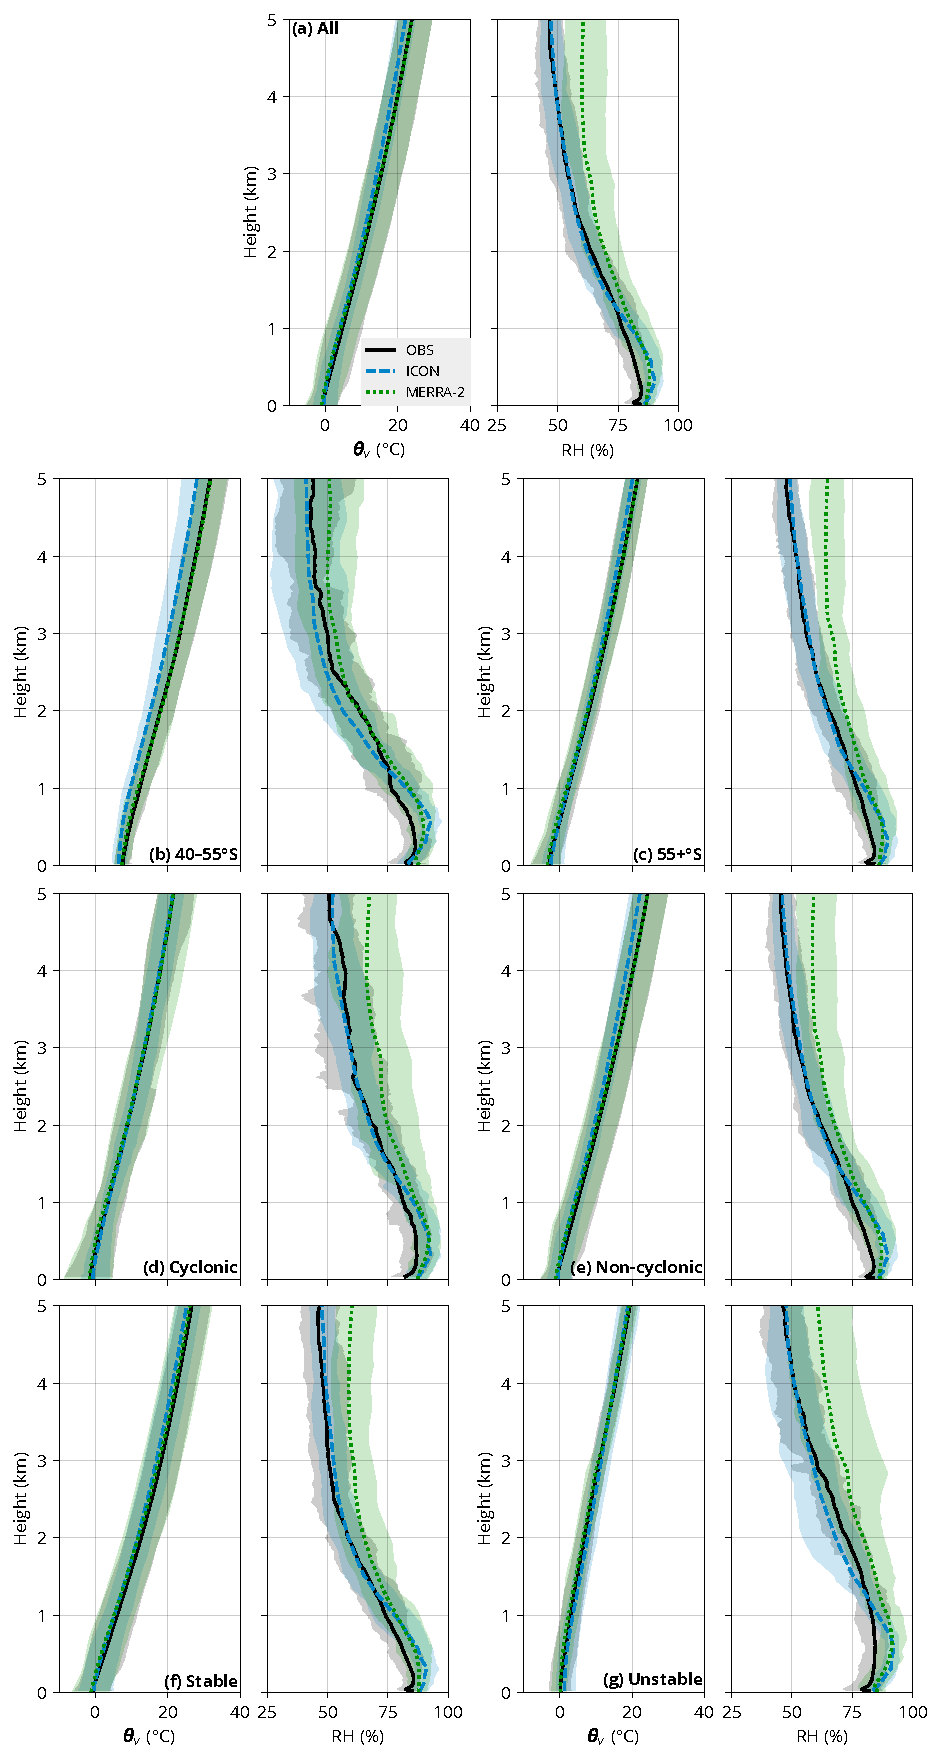
\includegraphics[width=0.72\textwidth]{img/theta_hur.pdf}
\caption{
Virtual potential temperature (virt.\ pot.\ temp.; $\theta_v$) and relative humidity (RH) determined from radiosonde launches and co-located profiles in ICON, ERA5, and MERRA-2 in subsets as in Fig.~\ref{fig:cloud-occurrence}. The solid lines are the average calculated from the averages of every individual voyage and station. The bands span the 16$^\mathrm{th}$--84$^\mathrm{th}$ percentiles, calculated from the distribution of the voyage and station averages. Shown is also the relative frequency of occurrence and the number of profiles in each subset.
}
\label{fig:potential-temperature}
\end{figure}

\subsection{Thermodynamic Profiles}

In order to link the cloud biases to the local physical conditions, we analyzed about 2300 radiosonde profiles south of 40°S from the 24 RV \emph{Polarstern} voyages, MARCUS, NBP1704, TAN1702, and TAN1802. Spatially and temporally colocated profiles were taken from ICON and the reanalyses. Because the time period covered by the ICON model output (2021--2024) was different from the time period covered by the observations (2010--2021), when comparing with the model, we first had to remap the observation time to model time by taking the same time relative to the start of the year. Consequently, we also had four virtual/model profiles (one for each year of 2021--2024) for each observed profile. The profiles were partitioned into the same subsets as above (Sections~\ref{sec:cloud-occurrence} and \ref{sec:cloud-cover}). Apart from relative humidity, we focus on comparing virtual potential temperature ($\theta_v$) due to its role in low-level tropospheric stability, being one of the primary factors affecting shallow convection and the associated low-level cloud formation and dissipation. The observed and model profiles of virtual potential temperature are shown in Fig.~\ref{fig:potential-temperature}.

Overall, the mean $\theta_v$ is accurate to less than 0.5~K in ICON and MERRA-2, except for ICON being colder by up to 2.5~K in the mid-to-high troposphere (less stable) (Fig.~\ref{fig:potential-temperature}a). Larger differences exist, however, in the 40--55°S zone, where ICON is colder by about 5 K at higher altitudes (Fig.~\ref{fig:potential-temperature}b). In other subsets, the bias is relatively small. MERRA-2 is very close to the observations, possibly due to a high accuracy of assimilation of this quantity. Notably, the variability of virtual potential temperature (as represented by the percentiles) is much smaller in ICON than in the observations. This indicates that the model's internal variability in the lower-tropospheric thermodynamic conditions in the SO is smaller than in reality.

Relative humidity displays much larger biases. In all subsets, ICON is too humid in the first 1~km by about 5\% but very accurate above, except for the 40--55°S zone and conditions of weak stability (Fig.~\ref{fig:potential-temperature}b, g), where it is too dry between about 1 and 3~km. MERRA-2, on the other hand, is more humid than observations at all altitudes and in all subsets, by up to about 20\% at~5 km. Even though the mean near-surface relative humidity is similar to the observations (Fig.~\ref{fig:potential-temperature}), the distribution in observation is more spread out across both high and low values, and thus observations have a greater prevalence of relative humidity close to 100\% and thus LCL located at the surface (Fig.~\ref{fig:cloud-occurrence}a). In our calculations, LCL is an exclusive function of near-surface temperature, near-surface relative humidity, and surface pressure.

\section{Limitations of this Study}
\label{sec:limitations}

Let us consider the main limitations of the presented results. The spatial coverage of our dataset does not include most parts of the Indian Ocean and Pacific Ocean sectors of the SO. Even though climatological features of the SO are typically relatively uniform zonally, variations exist, such as those related to the Antarctic Peninsula and the southern tip of South America. The voyages were mostly undertaken in the Austral summer months and only rarely in the winter months, due to the poor accessibility of this region during winter. Therefore, our results are likely representative of summer and, to a lesser extent, spring and autumn conditions.

The time period of ICON is relatively short, with only four full years of simulation available. Moreover, the simulation is free-running and ocean-coupled, which means that observations had to be temporally mapped to this time period (at the same time relative to the start of the year) for the comparison. For these reasons, one can expect the results to be slightly different due to reasons unrelated to model biases, such as different weather conditions, partially accounted for by the cyclone and stability subsetting, and the phase of climate oscillations such as the ENSO in the observations and the model. The interannual variability in cloud occurrence in ICON can be seen in Fig.~\ref{fig:cloud-occurrence-panel}, where each year in ICON is represented by a separate line. The interannual variability tends to be substantially smaller than the biases, and thus is unlikely to have a strong impact on the main findings.

Ground-based lidar observations are affected by attenuation by thick cloud layers, and for this reason the results are most representative of boundary layer clouds, while higher-level clouds are only occasionally visible to the lidar when boundary layer clouds are not present. Ground-based lidar observations can be regarded as superior to satellite lidar observations for low-level clouds, which are predominant in this region, while mid- and high-level clouds are better sampled by satellite observations \cite{mcerlich2021}. Near-surface lidar retrievals ($\sim$100~m) are affected by uncertainties related to incomplete overlap, signal saturation (dead time), and after-pulse effect corrections \cite{kuma2021}.

We have attempted to remove lidar profiles with precipitation, which could not be properly simulated with the lidar simulator (Section~\ref{sec:ann}). However, the approach was limited by the relatively low sensitivity of the ANN (65\%) and the fact that we had to choose a fixed threshold for surface precipitation flux in the model and reanalyses, which might not correspond to detection by the ANN applied to observations. Also, we made no attempt to remove profiles with precipitation not reaching the surface. The above reasons may result in an artificial bias in the comparison, even though we expect this to be much smaller than the identified model biases.

\section{Discussion and Conclusions}

We analyzed a total of about 2400 days of lidar and 2300 radiosonde observations from 31 voyages/campaigns and a subantarctic station, covering the Atlantic, Australian, and New Zealand sectors of the SO over the span of 10 years. This dataset, together with the use of a ground-based lidar simulator, provided a comprehensive basis for evaluating SO cloud and thermodynamic profile biases in the GSRM ICON and the ERA5 and MERRA-2 reanalyses. Our analysis provides a unique evaluation perspective different from satellite observations -- one that we argue is more suitable for evaluating boundary layer clouds, which are predominant in this region. Furthermore, we subsetted our dataset by low and high latitude bands, cyclonic activity, and stability in order to identify how these conditions influence the biases.

Our main finding corroborates previous findings of large boundary layer cloud biases in models and their subsequent effect on the radiative transfer. This also applies to the new GSRM ICON, but the biases are generally lower than in the reanalyses, despite the reanalyses having the advantage of assimilation of the observed meteorological conditions. The GSRM has, on the other hand, the advantage of a much higher spatial resolution and, to a limited extent, explicit calculation of traditionally subgrid-scale processes such as convection.

We show that relative to ERA5, the distribution and strength of cyclonic activity over the SO is well represented in ICON, but it displays lower values of LTS. The latter is also manifested in the radiosonde profile comparison, showing that the virtual potential temperature profiles in ICON are less stable than in the observations over low-latitude SO.

The 31 voyages and a station show remarkably similar biases in cloud occurrence by height in the lidar comparison, which indicates that common underlying causes for the biases exist regardless of longitude and season. ICON underestimates the total cloud fraction by about 10\%, with an overestimation of clouds below 2~km and an underestimation of clouds above 2~km. The reanalyses also underestimate the total cloud fraction by about 20\%. ERA5 overestimates cloud below 1~km but underestimates near-surface cloud or fog. ICON strongly overestimates the peak of cloud occurrence at about 500 m, which might be explained by the radiosonde comparison, showing that it is too moist at around this height. Similar to our results, \citeA{cesana2022} showed that CMIP6 models also tend to underestimate cloud occurrence above 2~km over the SO, although their analysis in this case was limited to liquid clouds.

Compared to lidar observations, the daily cloud cover tends to be about 1~okta lower in ICON and 2~oktas lower in the reanalyses. Conditions of weak stability are associated with some of the greatest biases, especially in ERA5. The models also underestimate the cloud cover very strongly in cyclonic conditions, which are very cloudy in the observations (8~oktas), but much less so in the models. Similarly, \citeA{mcerlich2023} found a 40\% underestimation of cloud liquid water in cyclones over the SO in ERA5, despite total column water vapor simulated much more accurately (5\% underestimation).

The radiosonde observations indicate that the LCL is too high in ICON and reanalyses, which is probably responsible for the higher peak of clouds in the models and the lack of near-surface clouds or fog. The radiosonde comparison, however, does not seem to explain cloud biases at higher altitudes. MERRA-2 is too moist at all heights. ICON also exhibits smaller internal variability than the radiosonde observations. Overall, the radiosonde comparison only partially explains the identified cloud biases, and other physical causes are likely contributing. This warrants further investigation, especially of ocean--atmosphere fluxes, shallow convection, and boundary layer turbulence. The lack of parameterized subgrid-scale convection in ICON could be a substantial issue even at the 5-km resolution.

The relationship between cloud biases and radiation has a number of notable features. Perhaps unsurprisingly, the reanalyses exhibit the too few, too bright bias previously identified in models. In our results, this is characterized by outgoing TOA SW radiation similar to or higher than in the satellite observations, while at the same time total cloud fraction is substantially underestimated relative to the ground-based lidar observations. This feature seems to be much more pronounced in ERA5 than in MERRA-2. On the other hand, this relationship is not present in ICON. This model generally predicts smaller outgoing TOA SW radiation and smaller total cloud fraction than observations, and the deficit of outgoing TOA SW radiation is approximately proportional to the deficit of the total cloud fraction. While this might be a welcome feature and an improvement over previous models, it does mean that the outgoing TOA SW radiation is overall underestimated instead of being compensated by a higher cloud albedo. This can, of course, lead to undesirable secondary effects such as overestimated solar heating of the sea surface, among other factors responsible for SO SST biases in climate models \cite{zhang2023,luo2023,hyder2018}. To some extent, the cloud albedo might be reduced in the model artificially by the application of an inhomogeneity factor to lower cloud liquid water in the radiative transfer calculations (Sec. \ref{sec:icon}).

The results imply that SO cloud biases are still a substantial issue even in the km-scale resolution ICON model, even though an improvement over the lower-resolution reanalyses is notable. More effort is needed to improve the model cloud simulations in this understudied region. However, this analysis suggests that the transition from models with parameterized convection and clouds to storm-resolving models might not solve these biases without additional effort. Evaluation of ocean--atmosphere heat, moisture, and momentum fluxes against in-situ observations over the SO and comparison of GSRM simulations against large-eddy simulations are two potential avenues for future research that could elucidate the physical mechanisms behind the biases, in addition to the more common efforts in SO cloud microphysics and precipitation evaluation.

\section*{Open Research Section}

The RV \emph{Polarstern} datasets are openly available on Pangaea (\url{https://pangaea.de}). The MARCUS and MICRE datasets are openly available from ARM (\url{https://www.arm.gov}). The MERRA-2 data are openly available from the NASA Goddard Earth Sciences (GES) Data and Information Services Center (DISC) (\url{https://disc.gsfc.nasa.gov/datasets?project=MERRA-2}). The ERA5 data are openly available from the Copernicus Climate Data Store (CDS) (\url{https://cds.climate.copernicus.eu}). The ICON data are available on the Levante cluster of the DKRZ (\url{https://www.dkrz.de/en/systems/hpc/hlre-4-levante}) after registration at \url{https://luv.dkrz.de/register/}. The CERES products are openly available from the project website (\url{https://ceres.larc.nasa.gov}) and the NASA Atmospheric Science Data Centre (\url{https://asdc.larc.nasa.gov/project/CERES}). The TAN1802 data are openly available on Zenodo (\url{https://doi.org/10.5281/zenodo.4060237}). The code for performing the presented analysis and precipitation detection is open-source and available at \url{https://github.com/peterkuma/icon-so-2024} and \url{https://github.com/peterkuma/alcf-precip}, respectively. The remaining voyage data are openly available on Zenodo (\url{https://doi.org/}).

\acknowledgments

PK, FB, and the nextGEMS project received funding from the European Union’s Horizon 2020 research and innovation program under a grant agreement no. 101003470. FB received funding from the Wenner-Gren Foundation and the Swedish e-Science Research Centre. The work of GM was supported by the United States (U.S.) Department of Energy Award DE-SC0021159. Supercomputing resources were provided by the DKRZ (project 1125 ICON-development) and the National Academic Infrastructure for Supercomputing in Sweden (allocation 2023/22-202). The data collection by the University of Canterbury was funded by the Deep South National Science Challenge Clouds and Aerosols project. Data collection on the AA15-16 voyages was funded by the Australian Antarctic Science project (grant no.~4292). We acknowledge the contribution of Thorsten Mauritsen to funding acquisition and project management. We acknowledge the RV \emph{Polarstern} datasets provided by the Alfred Wegener Institute and Pangaea, the AA15-16 dataset provided by the Australian Antarctic Division (AAD) and University of Canterbury (UC), the RV \emph{Tangaroa} datasets provided by the National Institute of Water and Atmospheric Research and UC, the NBP1704 dataset provided by the National Science Foundation, Cooperative Institute for Research in Environmental Sciences, University of Colorado and UC, the HMNZSW16 dataset provided by the Royal New Zealand Navy and UC, the MARCUS dataset provided by ARM and AAD, and the MICRE dataset provided by ARM, the Australian Bureau of Meteorology, and AAD. Technical, logistical, and ship support for MARCUS and MICRE were provided by the AAD through Australian Antarctic Science projects 4292 and 4387, and we thank Steven Whiteside, Lloyd Symonds, Rick van den Enden, Peter de Vries, Chris Young, Chris Richards, Andrew Klekociuk, John French, Terry Egan, Nick Cartwright, and Ken Barrett for all of their assistance. We thank the scientific staff, the crew, and everyone involved in collecting data on the voyages and stations, especially Gert König-Langlo, Holger Schmithüsen, Roger Marchand, Peter Guest, Kelly Schick, Jamie Halla, and Mike J. Harvey (†). We thank Loretta Preis for providing additional RV \emph{Polarstern} data. We acknowledge the ICON model output provided by the nextGEMS project, Deutscher Wetterdienst, Max-Planck-Institute for Meteorology, DKRZ, Karlsruhe Institute of Technology, and Center for Climate Systems Modeling; the reanalysis dataset ERA5 provided by the Copernicus Climate Change Service; MERRA-2 provided by the Global Modeling and Assimilation Office; CERES datasets provided by the NASA Langley Atmospheric Science Data Center Distributed Active Archive Center; and the Natural Earth dataset provided by naturalearthdata.com. Last but not least, we acknowledge the use of open-source software: Python, Cython \cite{behnel2011}, TensorFlow \cite{abadi2016}, Devuan GNU+Linux, parallel \cite{tange2011}, NumPy \cite{harris2020}, SciPy \cite{virtanen2020}, Matplotlib \cite{hunter2007}, cartopy \cite{cartopy}, pyproj, Inkscape, Bash, GNU Fortran, HDF \cite{folk1999}, and NetCDF \cite{rew1990}. We dedicate this study to the memory of Mike J. Harvey, who very substantially contributed to obtaining the atmospheric observations on the RV \emph{Tangaroa} voyages used in this study.

\bibliography{manuscript}

\end{document}
